%%%%%%%%%%%%%%%%%%%%%%%%%%%%%%%%%%%%%%%%%%%%%%%%%%%%%%%%%%%%%%%%%%%%%
%% This is a (brief) model paper using the achemso class
%% The document class accepts keyval options, which should include
%% the target journal and optionally the manuscript type. 
%%%%%%%%%%%%%%%%%%%%%%%%%%%%%%%%%%%%%%%%%%%%%%%%%%%%%%%%%%%%%%%%%%%%%
\documentclass[journal=jacsat,manuscript=article]{achemso}
\SectionNumbersOn
\usepackage{tikz} %Format quantum circuits
\usetikzlibrary{quantikz2}%Format quantum circuits

\usepackage{multicol}
\usepackage{graphicx}% Include figure files
\usepackage{graphicx}% Include figure files
\usepackage{dcolumn}% Align table columns on decimal point
\usepackage{bm}% bold math
%\usepackage[mathlines]{lineno}% Enable numbering of text and display math
%\linenumbers\relax % Commence numbering lines
\usepackage{pgffor}
\usepackage[utf8]{inputenc}
\usepackage[T1]{fontenc}
\usepackage{mathptmx}
\usepackage{listings}
\lstset{language=Python}
\usepackage{rotating} % Rotating table
\usepackage{caption}
\usepackage{subcaption}

\usepackage{color}
\usepackage{dcolumn} % decimal align in tables
\usepackage{bm} % bold math
\usepackage{graphicx}
\usepackage{multirow} % for table cells to span rows
\usepackage{pifont} % for checkmarks
\usepackage{epsfig}
\usepackage{amsmath} % matrix
% \usepackage{subfigure}
\usepackage{float}
\usepackage{booktabs}
\usepackage{tabularx}
\usepackage{natbib}
\usepackage{gensymb}
\setlength{\paperwidth}{8.5in}
\setlength{\paperheight}{11.0in}
\usepackage{rotating}
\usepackage{threeparttable}
\usepackage{comment}
%for corrections
\usepackage[normalem]{ulem}
\usepackage[hidelinks]{hyperref} % allows hyperlinking for references
%%%%%%%%%%%%%%%%%%%%%%%%%%%%%%%%%%%%%%%%%%%%%%%%%%%%%%%%%%%%%%%%%%%%%
%% Place any additional packages needed here.  Only include packages
%% which are essential, to avoid problems later. Do NOT use any
%% packages which require e-TeX (for example etoolbox): the e-TeX
%% extensions are not currently available on the ACS conversion
%% servers.
%%%%%%%%%%%%%%%%%%%%%%%%%%%%%%%%%%%%%%%%%%%%%%%%%%%%%%%%%%%%%%%%%%%%%
\usepackage[version=3]{mhchem} % Formula subscripts using \ce{}
\usepackage{xcolor}
\usepackage{amsmath,amssymb,amsthm}
\usepackage{mathtools,physics}
\usepackage{subcaption}
% \usepackage{titling}
%%%%%%%%%%%%%%%%%%%%%%%%%%%%%%%%%%%%%%%%%%%%%%%%%%%%%%%%%%%%%%%%%%%%%
%% If issues arise when submitting your manuscript, you may want to
%% un-comment the next line.  This provides information on the
%% version of every file you have used.
%%%%%%%%%%%%%%%%%%%%%%%%%%%%%%%%%%%%%%%%%%%%%%%%%%%%%%%%%%%%%%%%%%%%%
%%\listfiles

%%%%%%%%%%%%%%%%%%%%%%%%%%%%%%%%%%%%%%%%%%%%%%%%%%%%%%%%%%%%%%%%%%%%%
%% Place any additional macros here.  Please use \newcommand* where
%% possible, and avoid layout-changing macros (which are not used
%% when typesetting).
%%%%%%%%%%%%%%%%%%%%%%%%%%%%%%%%%%%%%%%%%%%%%%%%%%%%%%%%%%%%%%%%%%%%%
\newtheorem{theorem}{Theorem}[section]
\newtheorem{corollary}{Corollary}
\newtheorem{lemma}[theorem]{Lemma}
\newtheorem{proposition}{Proposition}
\newtheorem{conjecture}{Conjecture}
\newtheorem{definition}[theorem]{Definition}
\newtheorem{assumption}[theorem]{Assumption}
% \newtheorem{example}[theorem]{Example}
\newtheorem{example}{Example}[section]
\newtheorem{remark}{Remark}

% Add line numbers, as requested by Nature
\usepackage{lineno}
% \linenumbers


\newcommand*\mycommand[1]{\texttt{\emph{#1}}}
\newcommand{\noteg}[1]{\textcolor{red}{({Grier: #1})}}
\newcommand{\notek}[1]{\textcolor{darkspringgreen}{({Kostas: #1})}}

\def\myvdots{\ \vdots\ }
%%%% HELPER CODE FOR DEALING WITH EXTERNAL REFERENCES
% (from an answer by cyberSingularity at http://tex.stackexchange.com/a/69832/226)
%%%

\usepackage{xr-hyper}
%%%%%%%%%%%%%%%%%%%%%%%%%%%%%%%%%%%%%%%%%%%%%%%%%%%%%%%%%%%%%%%%%%%%%%%%
%----Helper code for dealing with external references----
% (by cyberSingularity at http://tex.stackexchange.com/a/69832/226)

\usepackage{xr}
\makeatletter

\newcommand*{\addFileDependency}[1]{% argument=file name and extension
	\typeout{(#1)}% latexmk will find this if $recorder=0
	% however, in that case, it will ignore #1 if it is a .aux or 
	% .pdf file etc and it exists! If it doesn't exist, it will appear 
	% in the list of dependents regardless)
	%
	% Write the following if you want it to appear in \listfiles 
	% --- although not really necessary and latexmk doesn't use this
	%
	\@addtofilelist{#1}
	%
	% latexmk will find this message if #1 doesn't exist (yet)
	\IfFileExists{#1}{}{\typeout{No file #1.}}
}\makeatother

\newcommand*{\myexternaldocument}[1]{%
	\externaldocument{#1}%
	\addFileDependency{#1.tex}%
	\addFileDependency{#1.aux}%
}
%------------End of helper code--------------

% put all the external documents here!
\myexternaldocument{SI}
\newcommand{\siref}[1]{S\ref{#1}}
%%%%%%%%%%%%%%%%%%%%%%%%%%%%%%%%%%%%%%%%%%%%%%%%%%%%%%%%%%%%%%%%%%%%%%%%


%%%%%%%%%%%%%%%%%%%%%%%%%%%%%%%%%%%%%%%%%%%%%%%%%%%%%%%%%%%%%%%%%%%%%
%% The document title should be given as usual. Some journals require
%% a running title from the author: this should be supplied as an
%% optional argument to \title.
%%%%%%%%%%%%%%%%%%%%%%%%%%%%%%%%%%%%%%%%%%%%%%%%%%%%%%%%%%%%%%%%%%%%%
\title{A Combinatorial Search of Parameterized Quantum Circuit Learning for Chemical Applications}
%%%%%%%%%%%%%%%%%%%%%%%%%%%%%%%%%%%%%%%%%%%%%%%%%%%%%%%%%%%%%%%%%%%%%
%% Meta-data block
%% ---------------
%% Each author should be given as a separate \author command.
%%
%% Corresponding authors should have an e-mail given after the author
%% name as an \email command. Phone and fax numbers can be given
%% using \phone and \fax, respectively; this information is optional.
%%
%% The affiliation of authors is given after the authors; each
%% \affiliation command applies to all preceding authors not already
%% assigned an affiliation.
%%
%% The affiliation takes an option argument for the short name.  This
%% will typically be something like "University of Somewhere".
%%
%% The \altaffiliation macro should be used for new address, etc.
%% On the other hand, \alsoaffiliation is used on a per author basis
%% when authors are associated with multiple institutions.
%%%%%%%%%%%%%%%%%%%%%%%%%%%%%%%%%%%%%%%%%%%%%%%%%%%%%%%%%%%%%%%%%%%%%
\author{Grier M. Jones}
\affiliation[UTSG ECE]{
	The Edward S. Rogers Sr. Department of Electrical and Computer Engineering, 
	University of Toronto, 
	10 Kings College Road, Toronto, Ontario, 
	Canada M5S 3G4}
\alsoaffiliation[UTM CHEM]{
	Department of Chemical and Physical Sciences, 
	University of Toronto Mississauga, 
	3359 Mississauga Road, Mississauga, Ontario, 
	Canada L5L 1C6}

\author{Nick Taylor}
\affiliation[UTSG ECE]{
	The Edward S. Rogers Sr. Department of Electrical and Computer Engineering, 
	University of Toronto, 
	10 Kings College Road, Toronto, Ontario, 
	Canada M5S 3G4}

\author{Viki Kumar Prasad}
\affiliation[UTSG ECE]{
	The Edward S. Rogers Sr. Department of Electrical and Computer Engineering, 
	University of Toronto, 
	10 Kings College Road, Toronto, Ontario, 
	Canada M5S 3G4}
\alsoaffiliation[UTM CHEM]{
	Department of Chemical and Physical Sciences, 
	University of Toronto Mississauga, 
	3359 Mississauga Road, Mississauga, Ontario, 
	Canada L5L 1C6}



\author{Ulrich Fekl}
\affiliation[UTM CHEM]{
	Department of Chemical and Physical Sciences, 
	University of Toronto Mississauga, 
	3359 Mississauga Road, Mississauga, Ontario, 
	Canada L5L 1C6}
\email{ulrich.fekl@utoronto.ca}

\author{Hans-Arno Jacobsen}
\affiliation[UTSG ECE]{
	The Edward S. Rogers Sr. Department of Electrical and Computer Engineering, 
	University of Toronto, 
	10 Kings College Road, Toronto, Ontario, 
	Canada M5S 3G4}
\email{jacobsen@eecg.toronto.edu}
%%%%%%%%%%%%%%%%%%%%%%%%%%%%%%%%%%%%%%%%%%%%%%%%%%%%%%%%%%%%%%%%%%%%%
%% Some journals require a list of abbreviations or keywords to be
%% supplied. These should be set up here, and will be printed after
%% the title and author information, if needed.
%%%%%%%%%%%%%%%%%%%%%%%%%%%%%%%%%%%%%%%%%%%%%%%%%%%%%%%%%%%%%%%%%%%%%
\abbreviations{}
\keywords{American Chemical Society, \LaTeX}

%%%%%%%%%%%%%%%%%%%%%%%%%%%%%%%%%%%%%%%%%%%%%%%%%%%%%%%%%%%%%%%%%%%%%
%% The manuscript does not need to include \maketitle, which is
%% executed automatically.
%%%%%%%%%%%%%%%%%%%%%%%%%%%%%%%%%%%%%%%%%%%%%%%%%%%%%%%%%%%%%%%%%%%%%
\newcommand{\R}{\mathbb{R}}


\begin{document}
	
	
\section{Dataset}	
The function fitting dataset consists of a noisy linear (Fig. \ref{fig:linear_train_vs_test}), quadratic (Fig. \ref{fig:quadratic_train_vs_test}), and sine (\ref{fig:sine_train_vs_test}) function.  
For each function, 90 points are generated, where 80 are used for training set and 10 for the test set.
This dataset is used for calibration of the 168 PQCs, along with providing additional insights into the effects of circuit depth, training set size, and error mitigation on model performance.


\begin{figure}[H]
	\centering
	\begin{subfigure}[b]{0.3\textwidth}
			\centering
			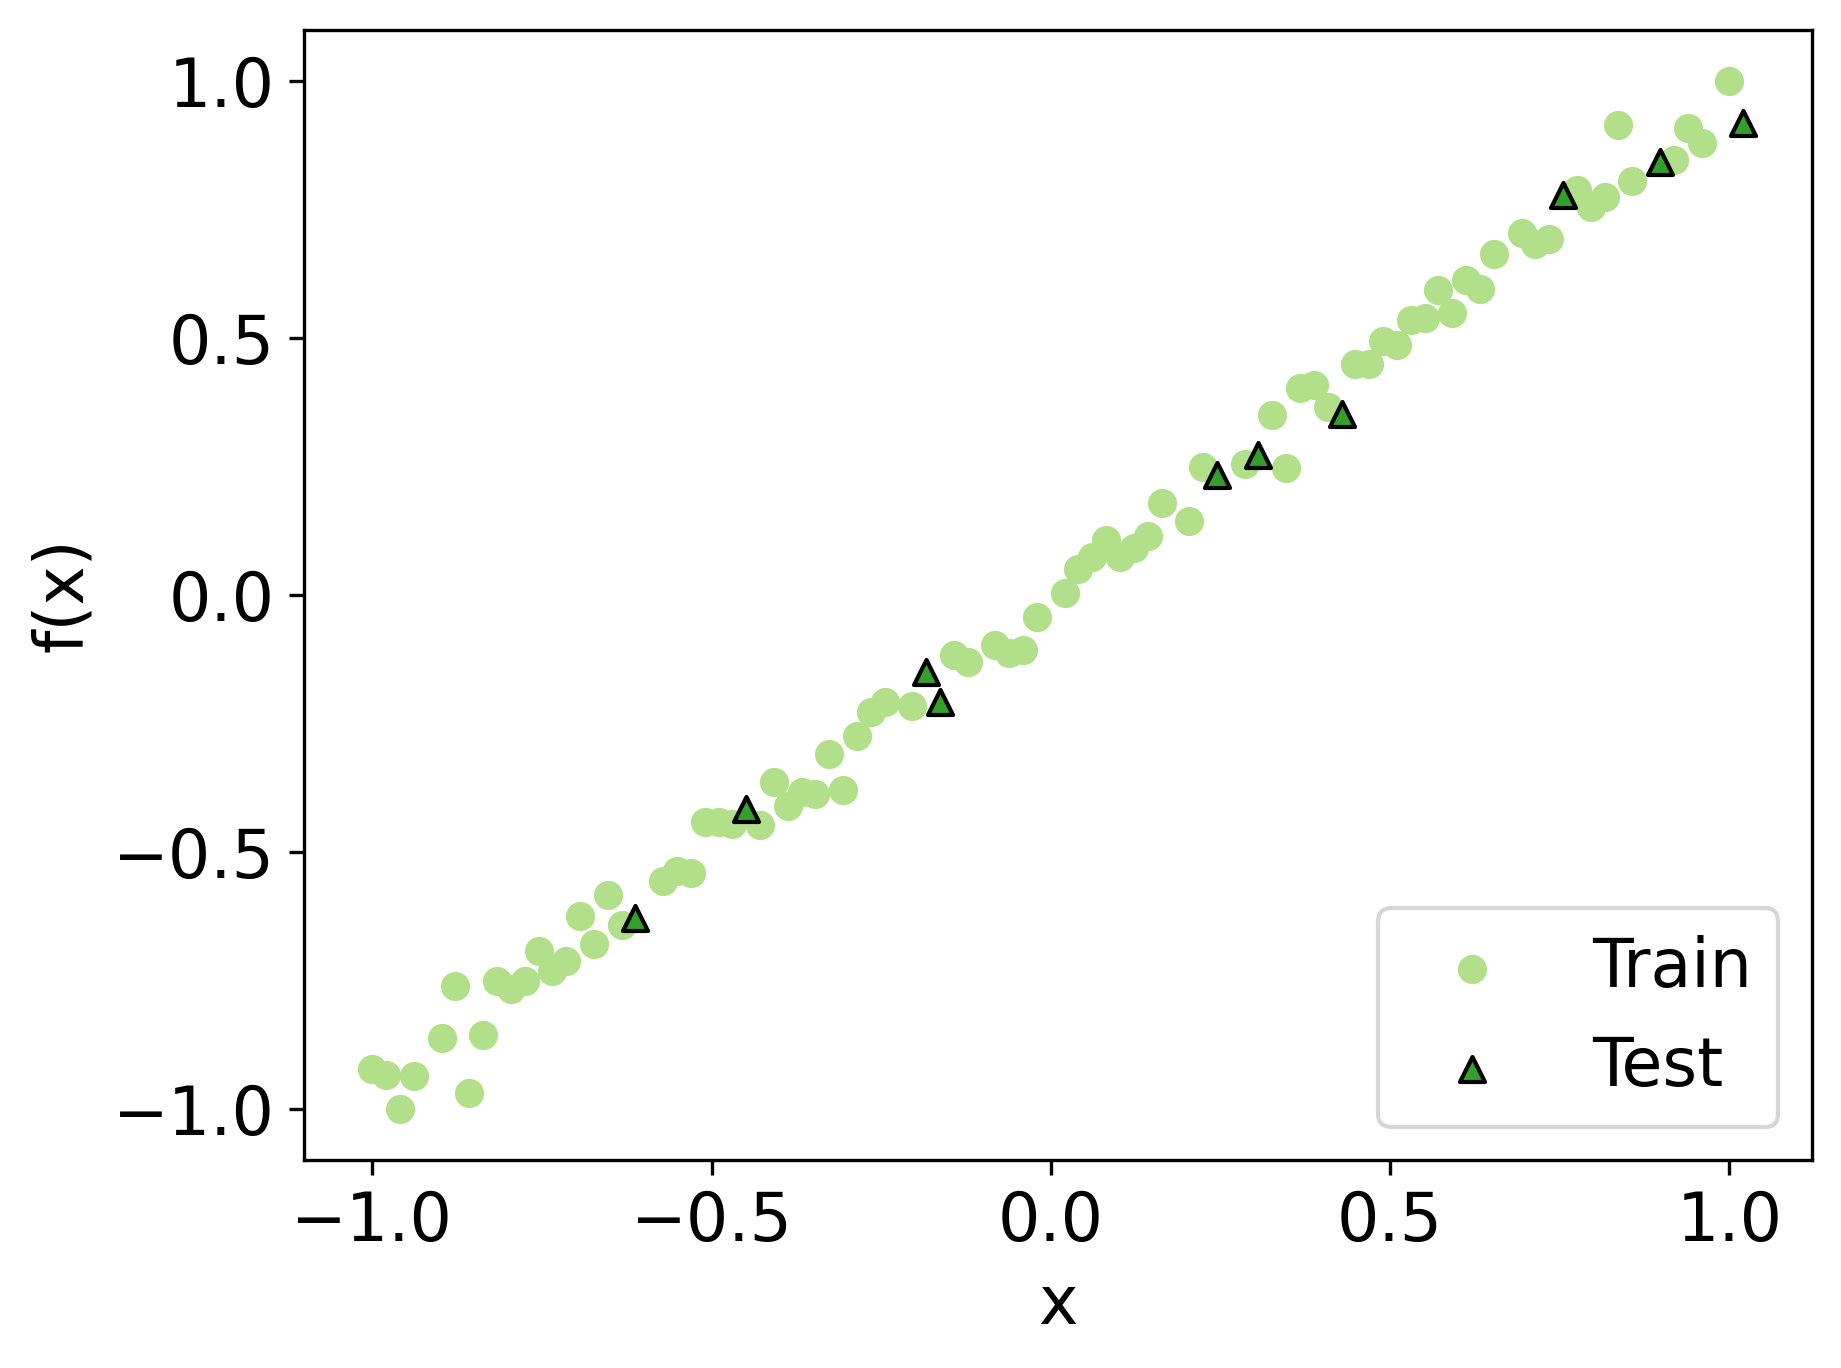
\includegraphics[width=\textwidth]{../images/Function_Fitting/function_dataset/linear_train_vs_test.png}
			\caption{}
			\label{fig:linear_train_vs_test}
		\end{subfigure}
	\hfill
	\begin{subfigure}[b]{0.3\textwidth}
			\centering
			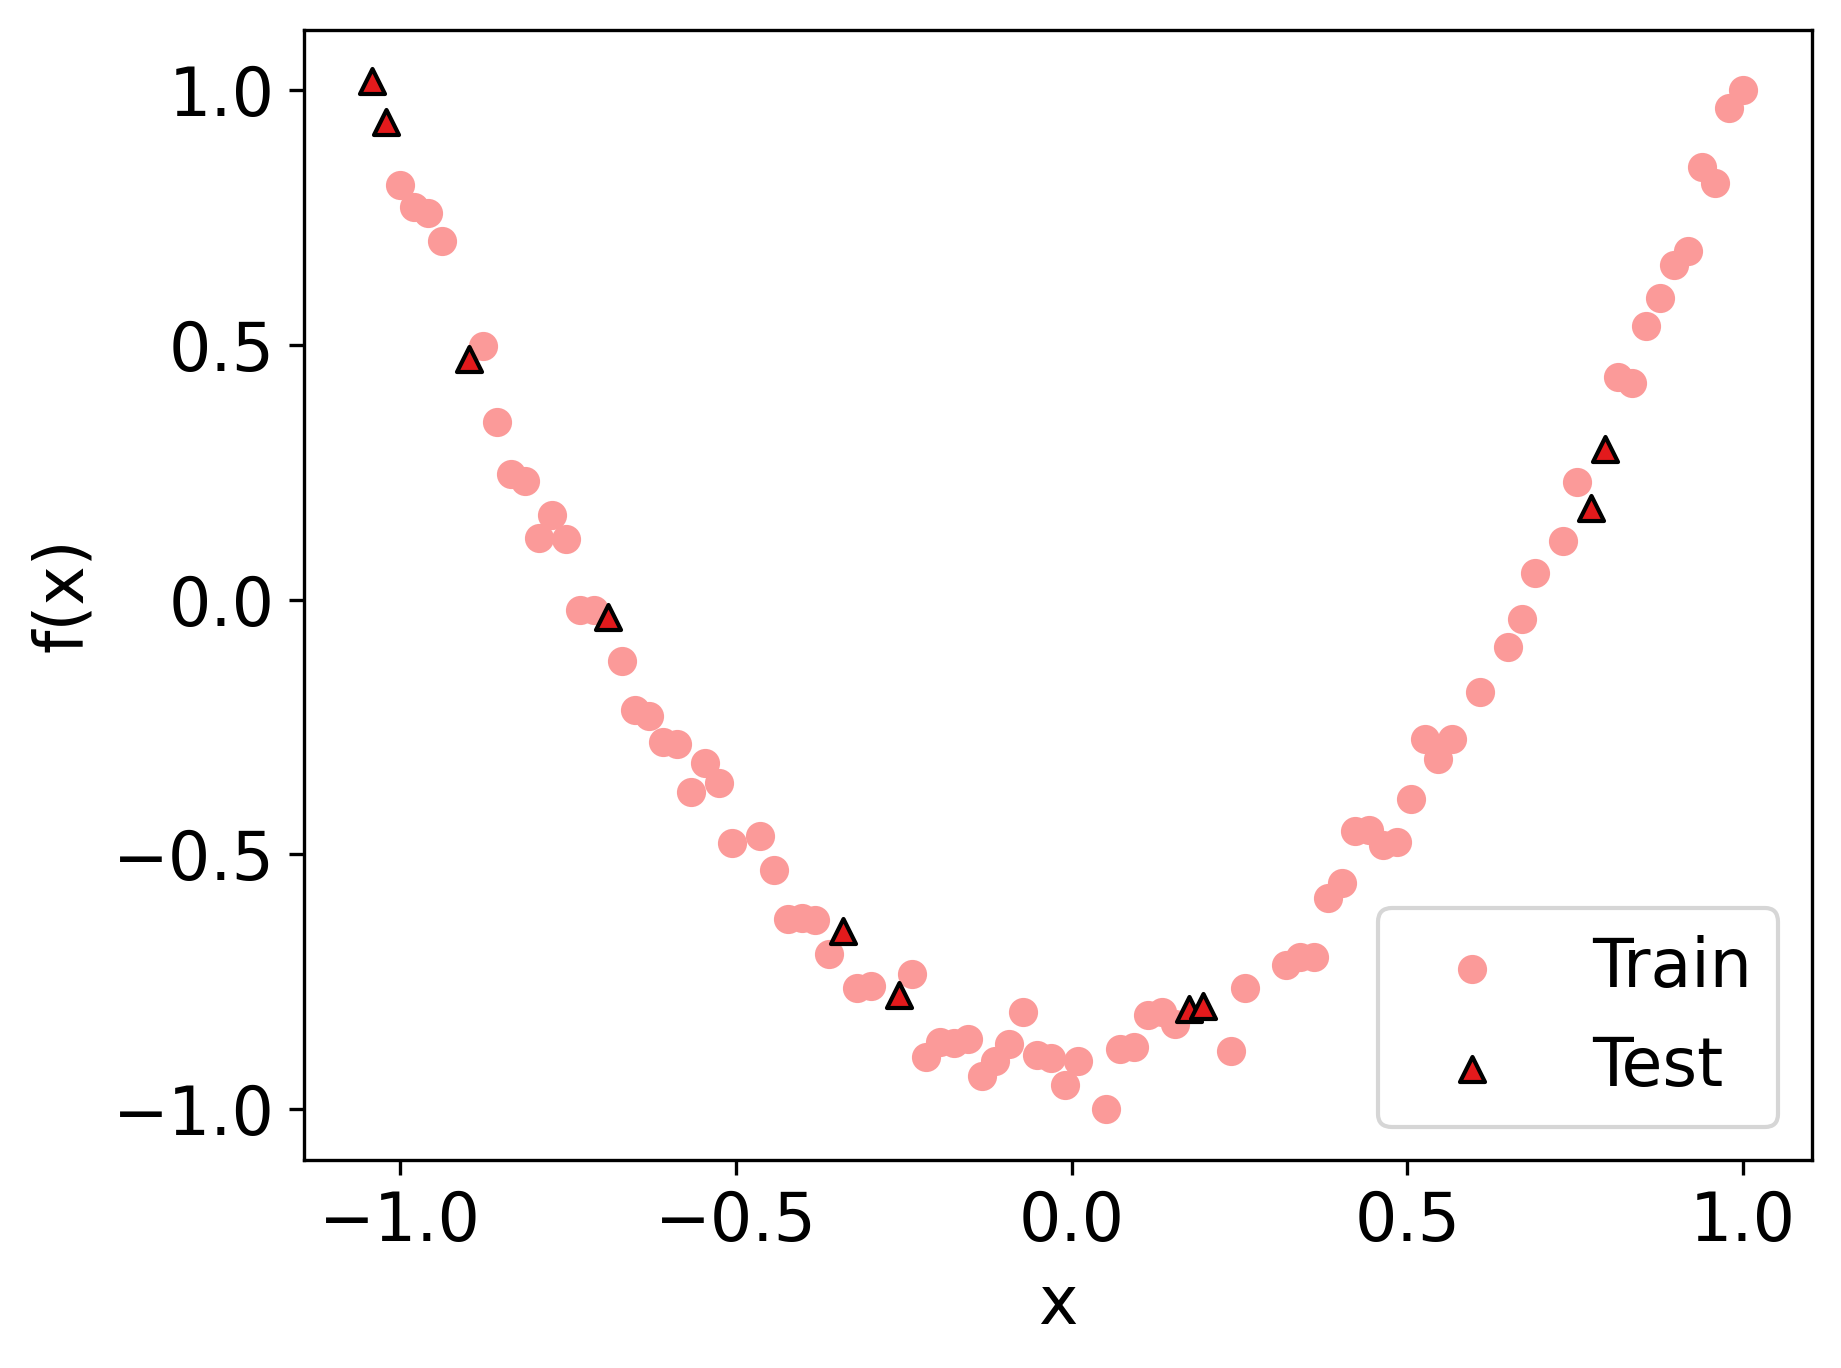
\includegraphics[width=\textwidth]{../images/Function_Fitting/function_dataset/quadratic_train_vs_test.png}
			\caption{}
			\label{fig:quadratic_train_vs_test}
		\end{subfigure}
	\hfill
	\begin{subfigure}[b]{0.3\textwidth}
			\centering
			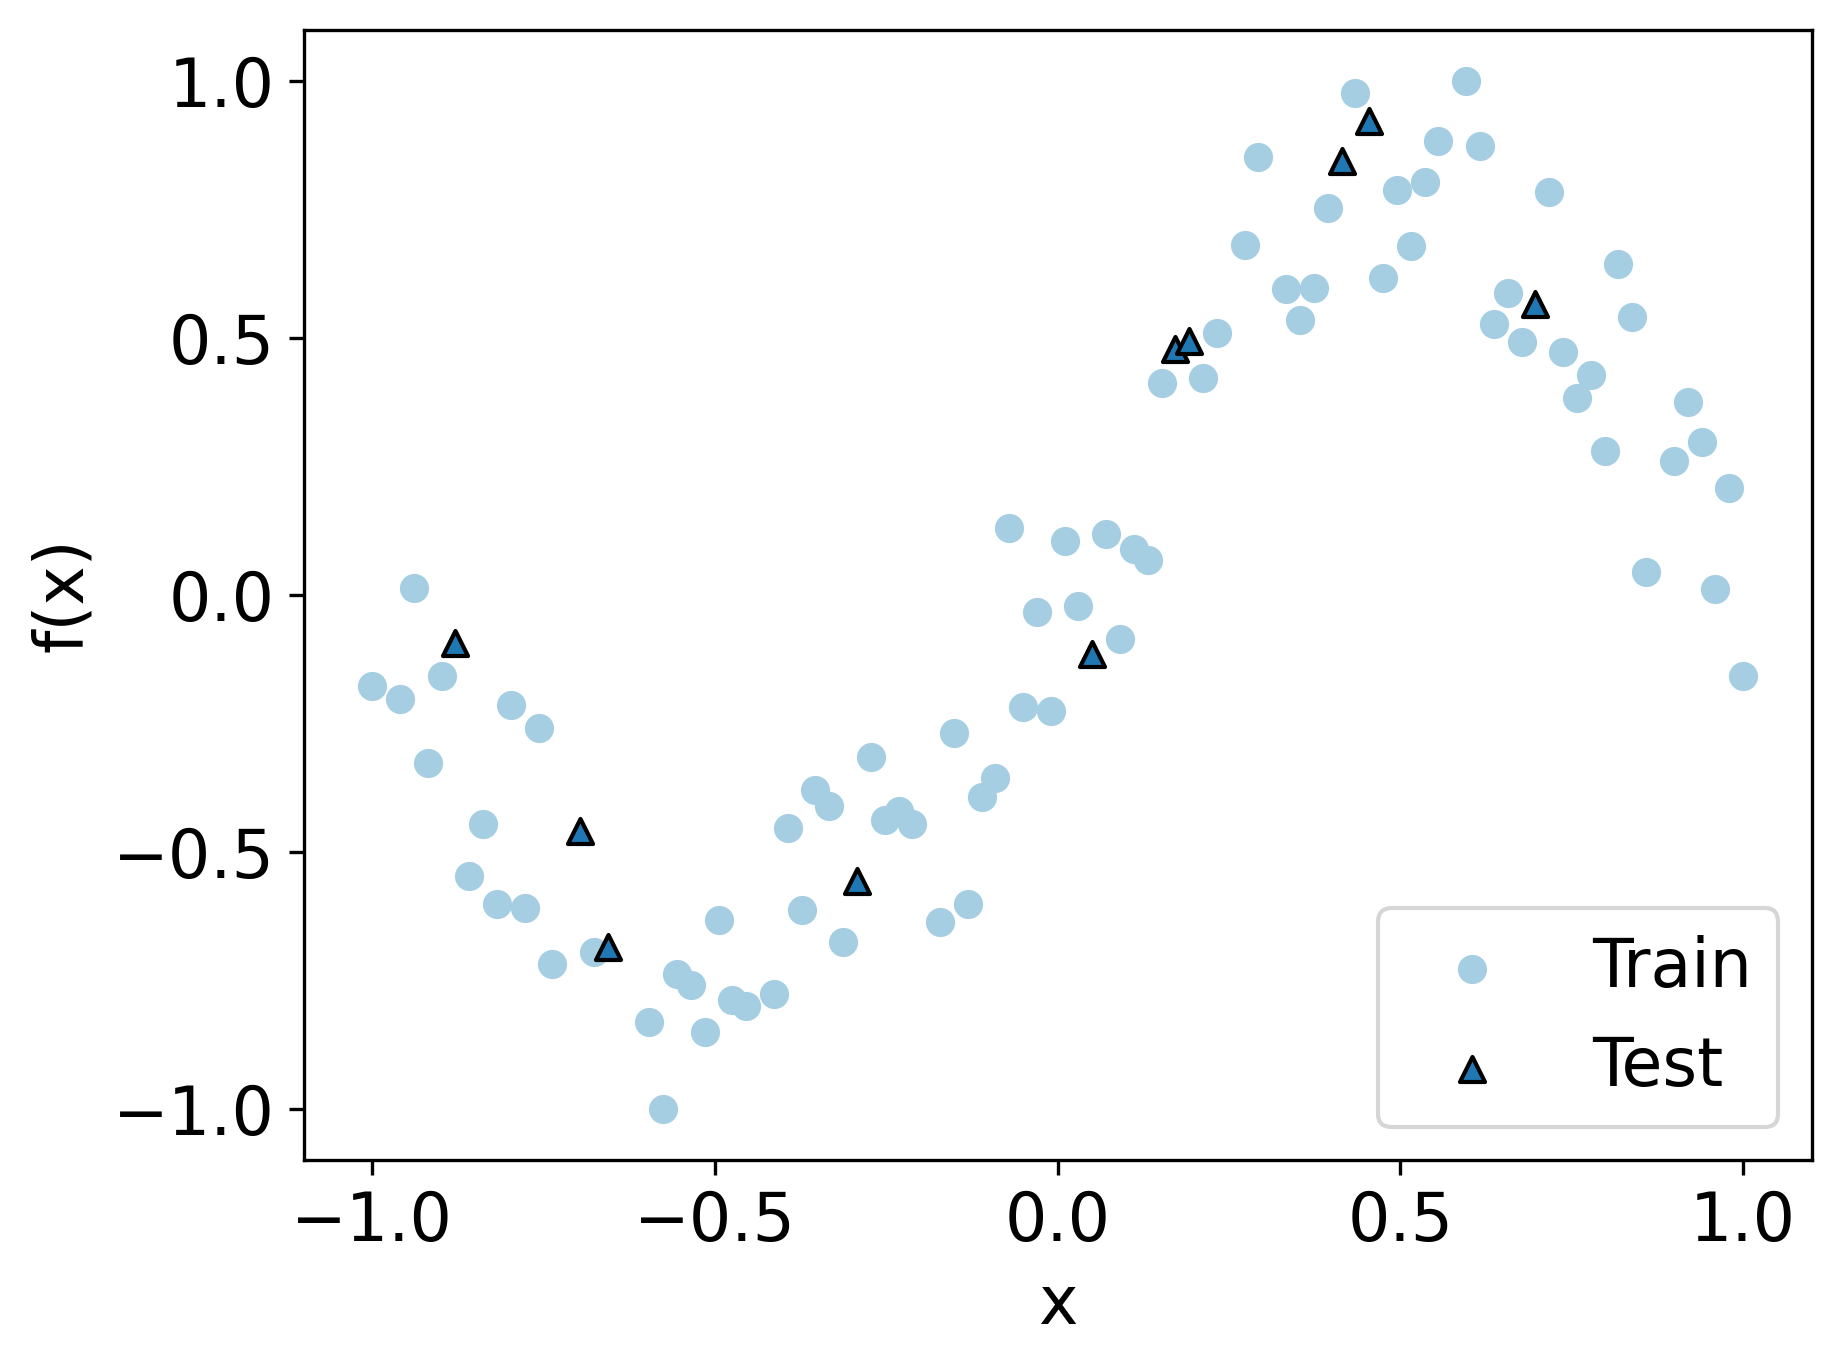
\includegraphics[width=\textwidth]{../images/Function_Fitting/function_dataset/sine_train_vs_test.png}
			\caption{}
			\label{fig:sine_train_vs_test}
		\end{subfigure}
	\caption{The function fitting dataset which consists of 90 total points, 80 for training and 10 used for testing, for the (a) linear, (b) quadratic, and (c) sine functions.}
	\label{fig:train_vs_test}
\end{figure}


\section{Function Fitting}
To calibrate the PQCs, we perform an initial study of the 168 encoder-ansatz pairs using both 5 and 16 qubits.
Individual heat maps showing the performance of the encoder-ansatz pairs and box plots showing the overall statistics for each encoder and ansatz are shown for the 5 and 16 qubit models in SI Section \siref{section:si_functionfitting}.


Starting with the five qubit function fitting, we found that out of the
168 encoder-ansatz pairs, for the linear function (SI Fig. \siref{fig:linear_heatplots}) is is A1\_ESU2 with a train and test R$^{2}$ of 0.9886 and 0.9893, respectively.
Box plots for the encoders (left) and variational layers (right) are shown in SI  Fig. \siref{fig:linear_boxplots}, where, the best encoder is IQP, with a mean R$^{2}$ of 0.8434, and best ansatz layer Full-CRX, with a mean R$^{2}$ of 0.7562.
For the quadratic function, the best encoder-ansatz pair is A1-A1-CNOT\_Full-CRX with a train and test R$^{2}$ of 0.8809 and 0.7309, respectively, as shown in SI Fig \siref{fig:quadratic_heatplots}.
On average the best encoder is A1-A1-CNOT with an R$^{2}$ of 0.5541 and best variational layer is Full-CRX with an R$^{2}$ of 0.5958 (SI  Fig. \siref{fig:quadratic_boxplots}).
For the sine function, SI  Fig. \siref{fig:sine_heatplots}, M-M-CZ\_Full-CRX is the best encoder-ansatz pair with a train and test R$^{2}$ of 0.8887 and 0.9081, respectively.
As shown in SI  Fig. \siref{fig:sine_boxplots}, the best encoder is M with an average R$^{2}$ of 0.6456 and best variational layer is Full-CRX with a mean R$^{2}$ of 0.7551.
Across all three five qubit function fitting datasets, on average, the best encoders are M-A2-CZ with an average R$^{2}$ of 0.4776 (Fig. \ref{fig:five_feature_function_fitting_boxplots} left) and ansatz is Full-CRX with an average R$^{2}$ of 0.7023 (Fig. \ref{fig:five_feature_function_fitting_boxplots} right).

For the sixteen qubit function fitting evaluation of the 168 encoder-ansatz pairs, we found that, similarly to the five qubit data, for the linear function the best pair is A1\_ESU2 with train and test R$^{2}$s of 0.9886 and 0.9893, respectively, as highlighted in SI Fig. \siref{fig:sixteenlinear_heatplots}.
Like the five qubit data, the best encoder is also IQP with an average R$^{2}$ of 0.7800 (SI Fig. \siref{fig:sixteenlinear_boxplots} left), while the best ansatz varies from the five qubit data, Full-Pauli-CRZ with a mean R$^{2}$ of 0.3947 (SI Fig. \siref{fig:sixteenlinear_boxplots} right).
The A1-A1-CZ\_Modified-Pauli-CRX encoder-ansatz pair has the best overall model performance, highlighted in SI Fig. \siref{fig:sixteenquadratic_heatplots}, where the training set has an R$^{2}$ of 0.8415 and the test set has an R$^{2}$ of  0.7722.
As demonstrated in SI Fig. \siref{fig:sixteenquadratic_boxplots}, the best encoders and ans\"{a}tze are A1-A1-CNOT and Full-Pauli-CRX, with mean R$^{2}$s of 0.5759 and 0.4474, respectively.
For the last sixteen qubit dataset, the sine function data (SI Fig. \siref{fig:sixteensine_heatplots}), the best encoder-ansatz pair is A1-A1-CZ\_Full-Pauli-CRZ	with an R$^{2}$ of 0.8147 for the training set and an R$^{2}$ of 0.8626	for the test set.
SI Fig. \siref{fig:sixteensine_boxplots} highlights that the best encoder is M with a mean R$^{2}$ of 0.5824 and best ansatz, on average, is Full-Pauli-CRZ with an R$^{2}$ of 0.4881.
Across all three function fitting datasets, the sixteen qubit data varies where the best encoders are IQP with an average R$^{2}$ of 0.4506 and ans\"{a}tze is Full-Pauli-CRZ with an average R$^{2}$ of 0.4393.

\begin{figure}[H]
	\centering
	\begin{subfigure}[b]{0.49\textwidth}
		\centering
		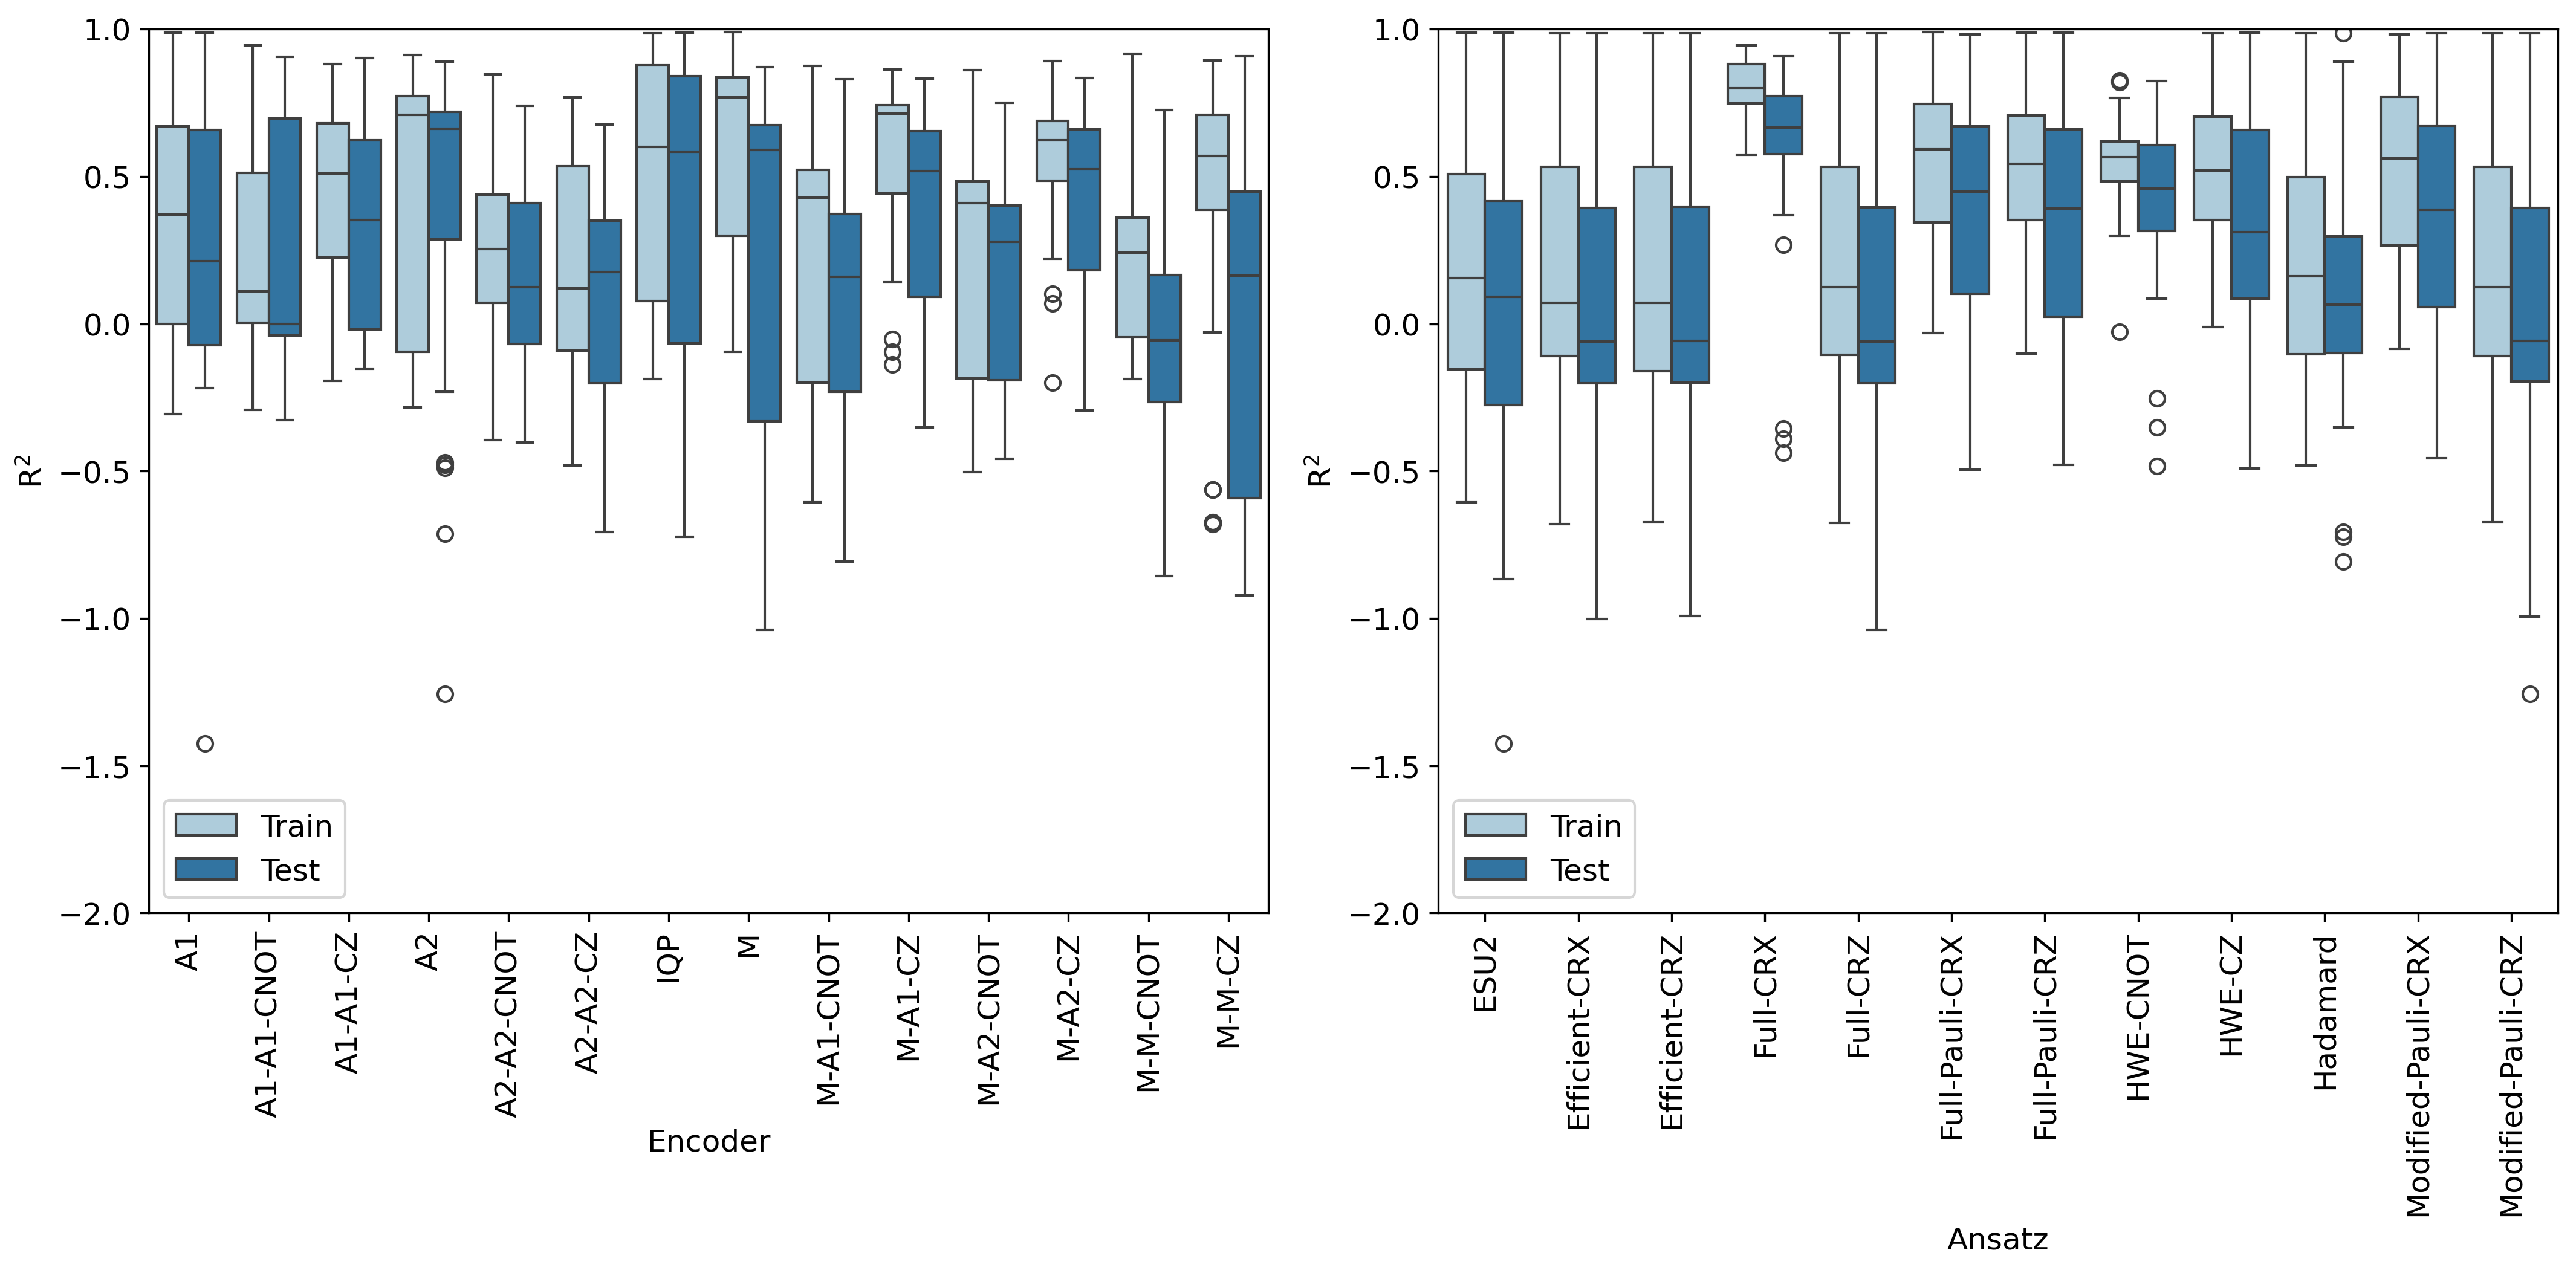
\includegraphics[width=\textwidth]{../images/Function_Fitting/fivequbit/five_feature_function_fitting_boxplots.png}
		\caption{}
		\label{fig:five_feature_function_fitting_boxplots}
	\end{subfigure}
	\hfill		
	\begin{subfigure}[b]{0.49\textwidth}
		\centering
		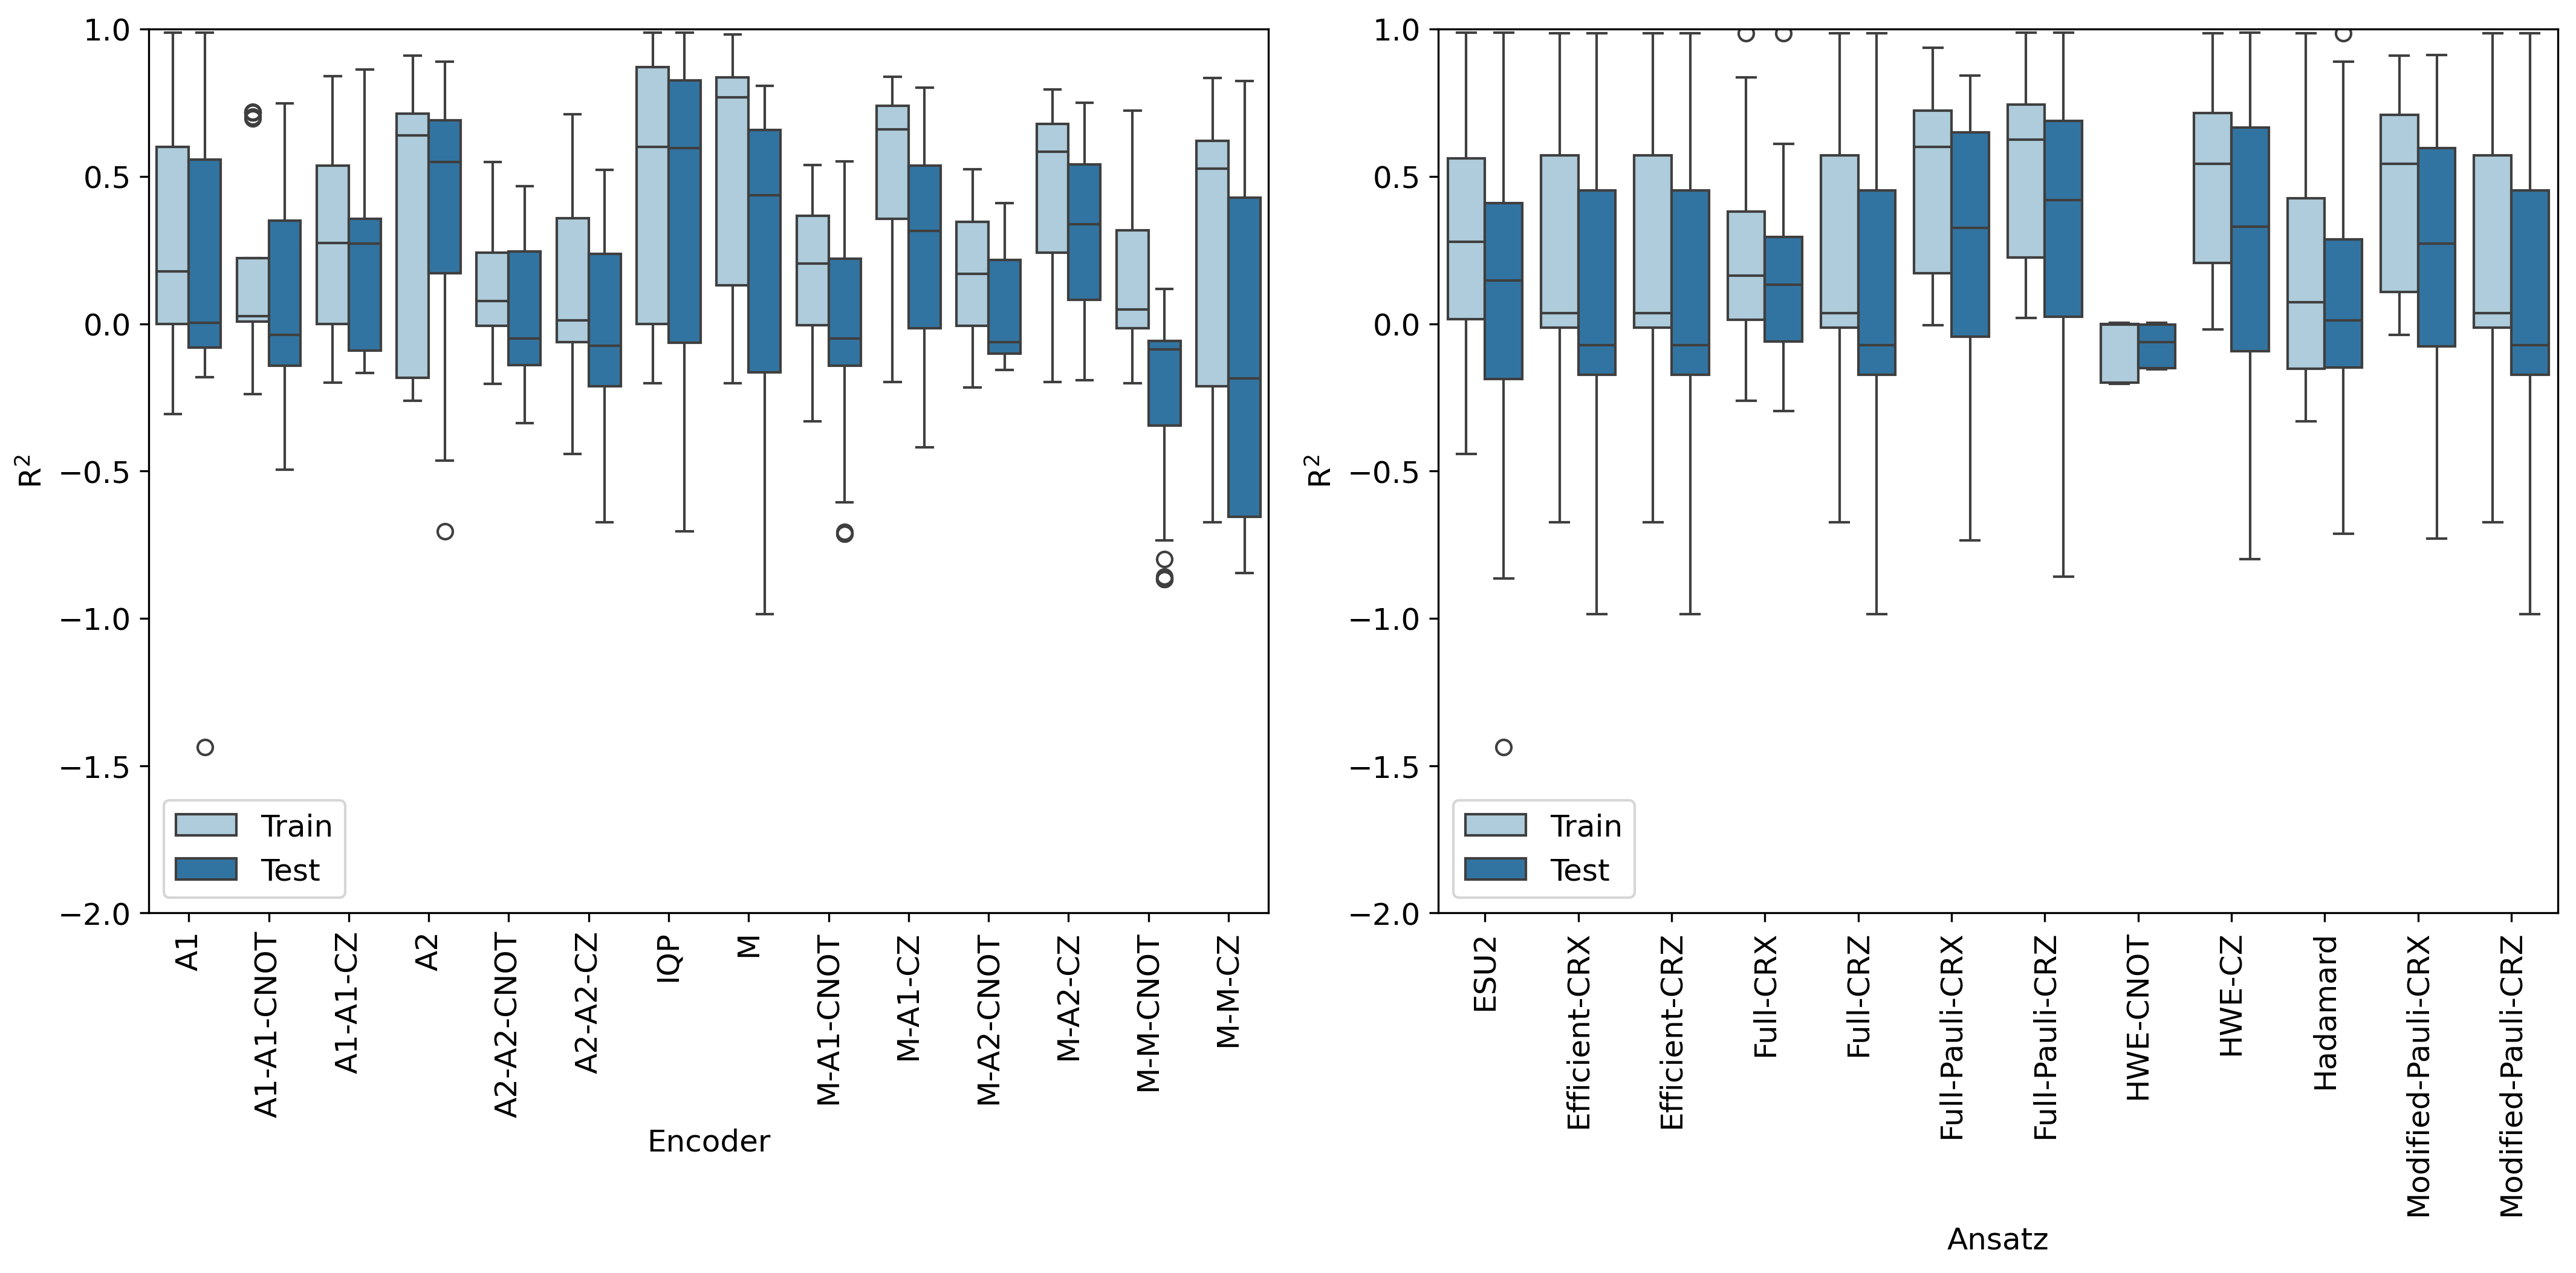
\includegraphics[width=\textwidth]{../images/Function_Fitting/sixteenqubit/sixteen_feature_function_fitting_boxplots.png}
		\caption{}
		\label{fig:sixteen_feature_function_fitting_boxplots}
	\end{subfigure}
	\hfill		
	\caption{The combined performance of all three function fitting datasets for both the (a) five and (b) sixteen qubit models is evaluated using the R$^{2}$ (y-axis) versus the encoders (left) and ans\"{a}tze (right).}
	\label{fig:function_fitting_boxplots}
\end{figure}


Following the initially analysis of the performance of the 168 PQCs using both five and sixteen qubits, we experimented with the effect of the re-upload depth (RUD) and number of ansatz layers (AL) using the sixteen qubit circuits.
We chose to use the sixteen qubit circuits over the five qubit circuits since these circuits have complexity more similar to when the circuits are used for the chemical dataset in terms of the number of parameters and optimization times.
From the initial 168 PQCs, for each function fitting dataset, we choose the five best (top row), five median (middle row), and five worst (bottom row) circuits to see the effects of increasing the RUD and AL on model performance as shown in Figs. \ref{fig:16qubit_Linear_RUD_AL}, \ref{fig:16qubit_Quadratic_RUD_AL}, and  \ref{fig:16qubit_Sine_RUD_AL}.
For the linear (Fig. \ref{fig:16qubit_Linear_RUD_AL}), quadratic (\ref{fig:16qubit_Quadratic_RUD_AL}), and sine (Fig. \ref{fig:16qubit_Sine_RUD_AL}) data, some generalities arise for the five best circuits. 
We see that for these circuits, increasing the number of AL from 1 to 3 or 5 improves model performance more than RUD.
For the median performers, the RUD improves model performance more than the ansatz layers.
And lastly, for the worse performers a general trend does not exist and increasing the RUD and AL depends on the dataset and circuit architecture. 


% Commented this out because it is not useful for the overall discussion
%While an increase in the circuit depth, either by increasing the RUD or AL, is associated with an increase in model performance this is also associated with an increased computational cost. 
%In Figs. \ref{fig:linear_circuitdepth_vs_R2}, \ref{fig:quadratic_circuitdepth_vs_R2}, and \ref{fig:sine_circuitdepth_vs_R2} we  highlight this trade-off, where the x-axes denote circuit depth, y-axis denotes the R$^{2}$, and the median train and test R$^{2}$ are shown in red and blue, respectively, for all 15 circuits. 
Despite these trends, we found that for the linear function, the best performing model is IQP\_Full-Pauli-CRZ  with a RUD and AL of 1.
This circuit also has a training and test R$^{2}$ of 0.9883 and 0.9891, respectively, and a depth of 95.
Unlike the best linear circuit, the best circuits for both the quadratic and sine data, IQP\_Full-Pauli-CRX	 and A2\_HWE-CZ, respectively,  benefit from an increased RUD, with the best models having a RUD of 5 and AL of 1.
These two circuits differ in depth and performance, with the IQP\_Full-Pauli-CRX for the quadratic data having a circuit depth of 520, training R$^{2}$ of 0.9817, and test R$^{2}$ of 0.9609 and the A2\_HWE-CZ circuit for the sine data having a depth of 105 , training R$^{2}$ of 0.9156, and test R$^{2}$ of 0.9576.
Following these insights, we applied these circuits for analyzing the effects of the training set size on model performance using learning curves and the effects of error mitigation using noisy simulation.


\begin{figure}[H]
	\centering	
	\begin{subfigure}[b]{0.49\textwidth}
		\centering
		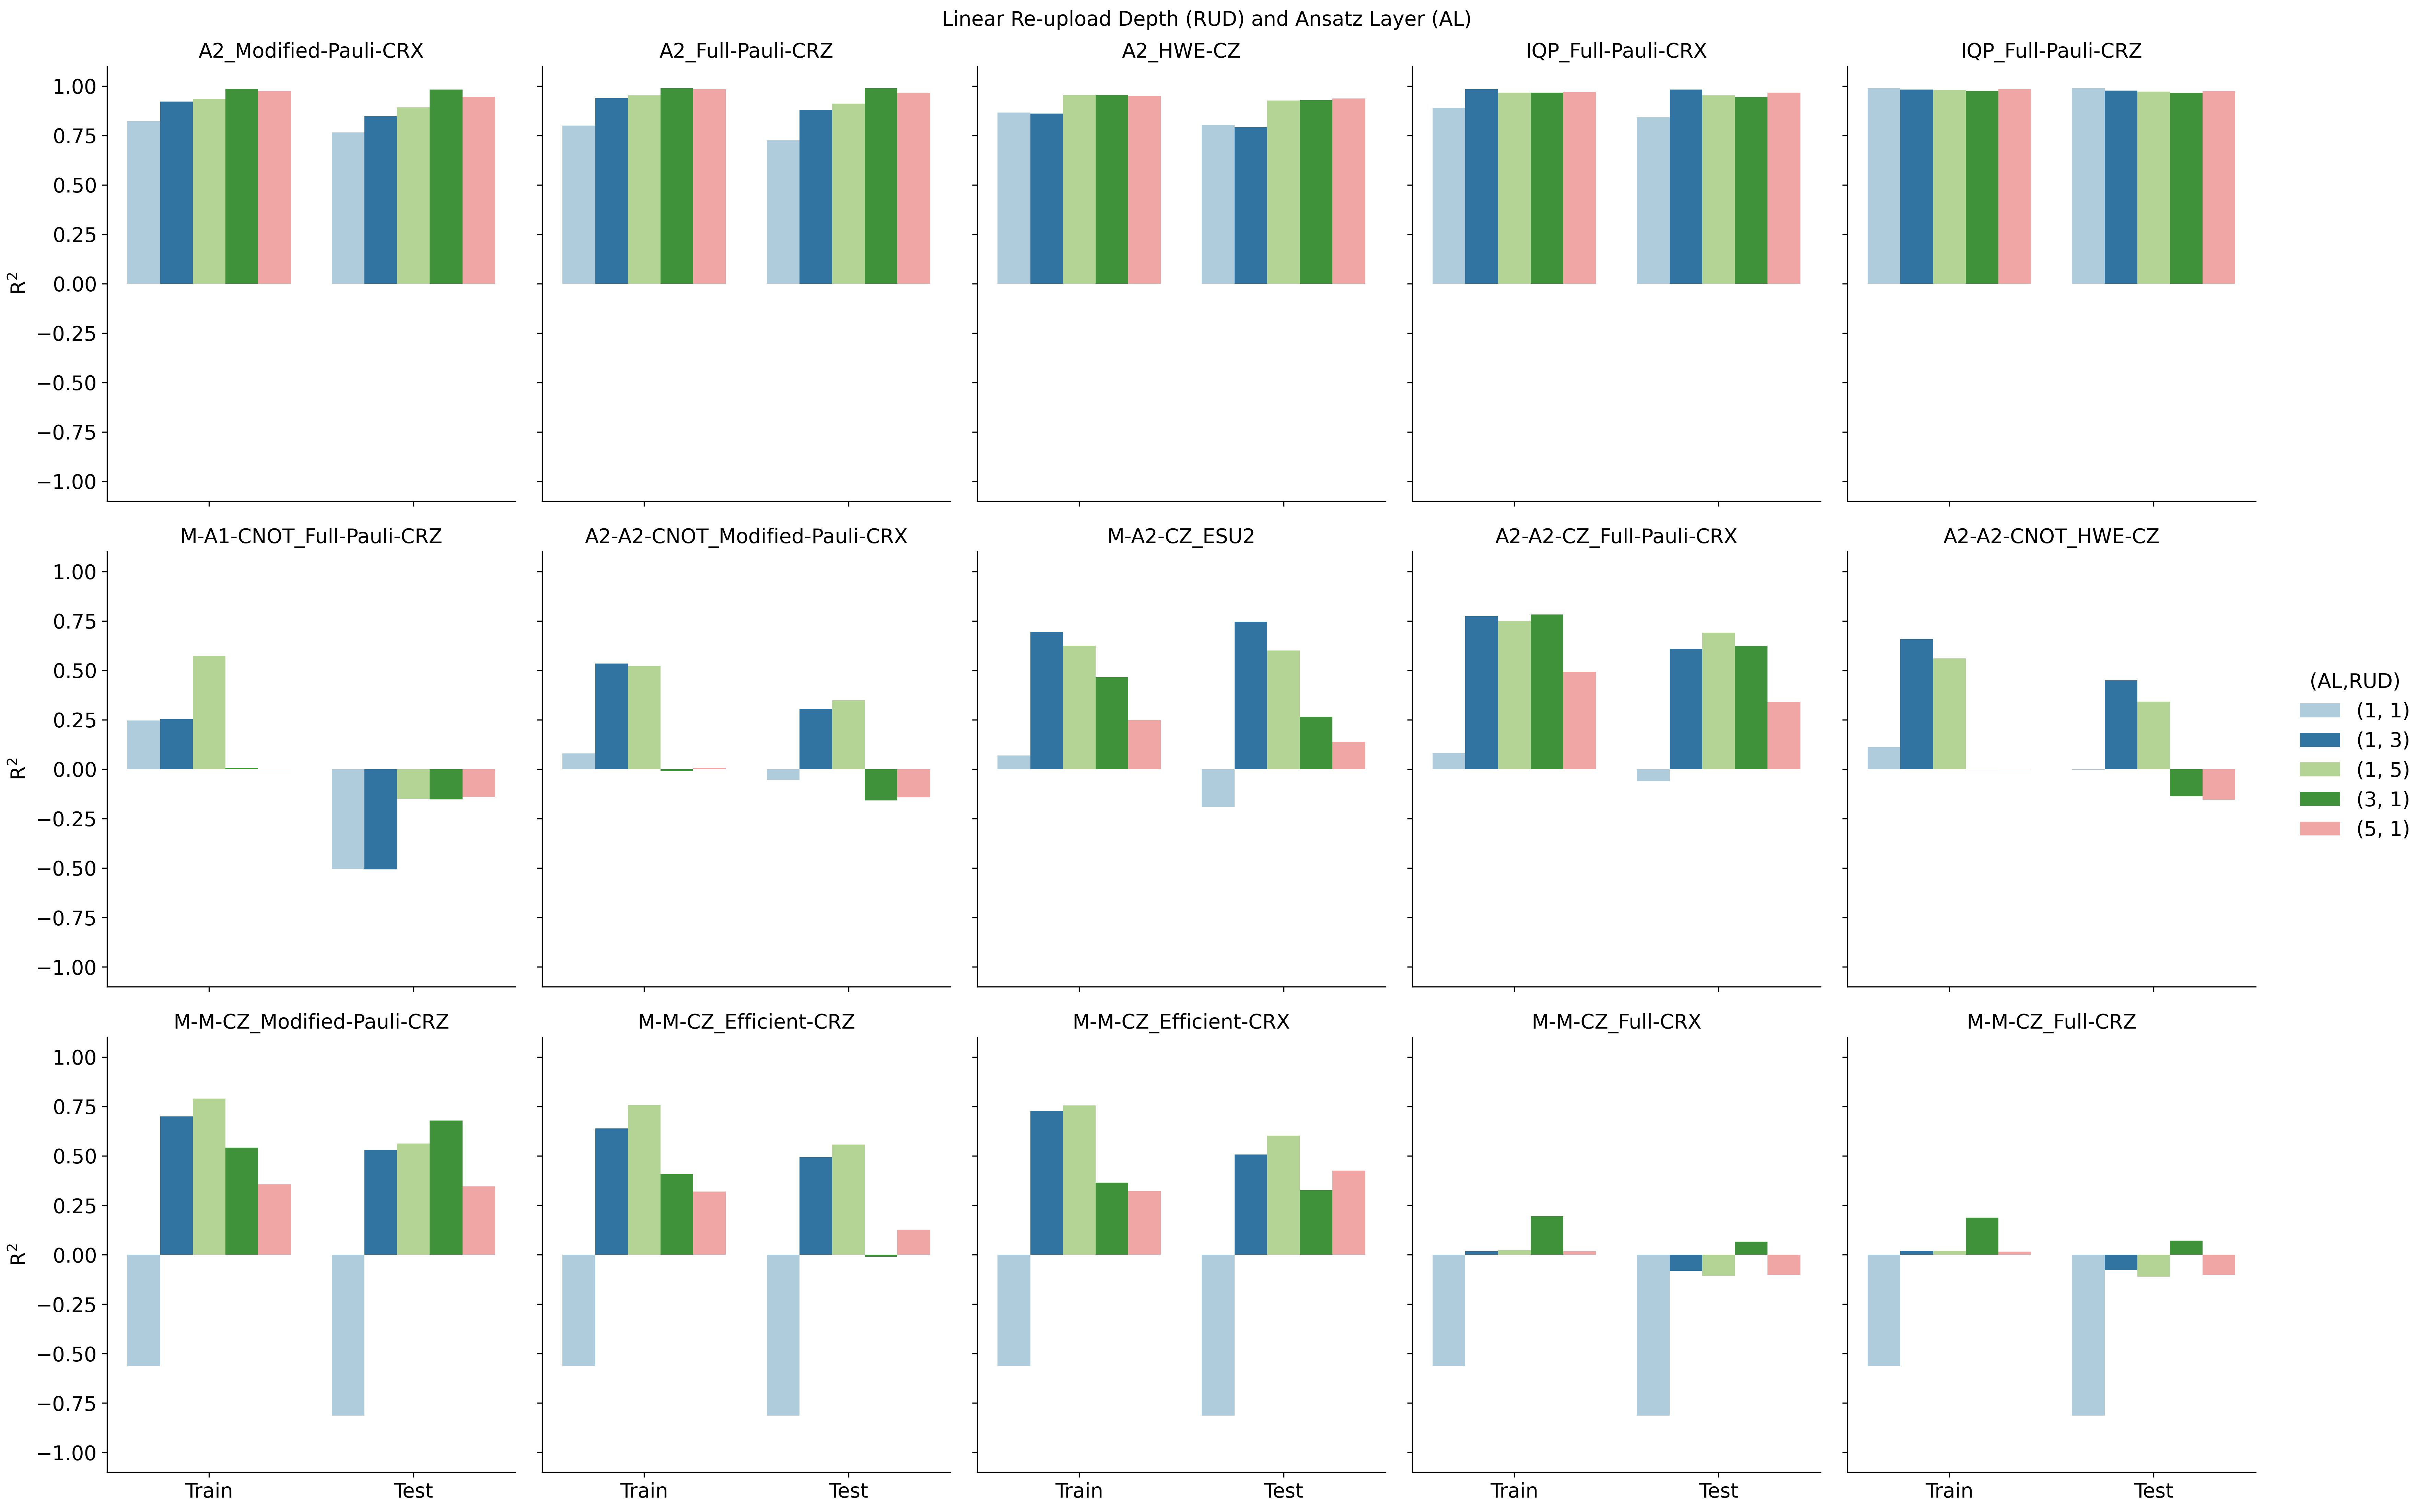
\includegraphics[width=\linewidth]{../images/Function_Fitting/sixteenqubit/16qubit_Linear_RUD_AL}
		\caption{}
		\label{fig:16qubit_Linear_RUD_AL}
	\end{subfigure}
	\hfill	
	%	\begin{subfigure}[b]{0.49\textwidth}
		%		\centering
		%		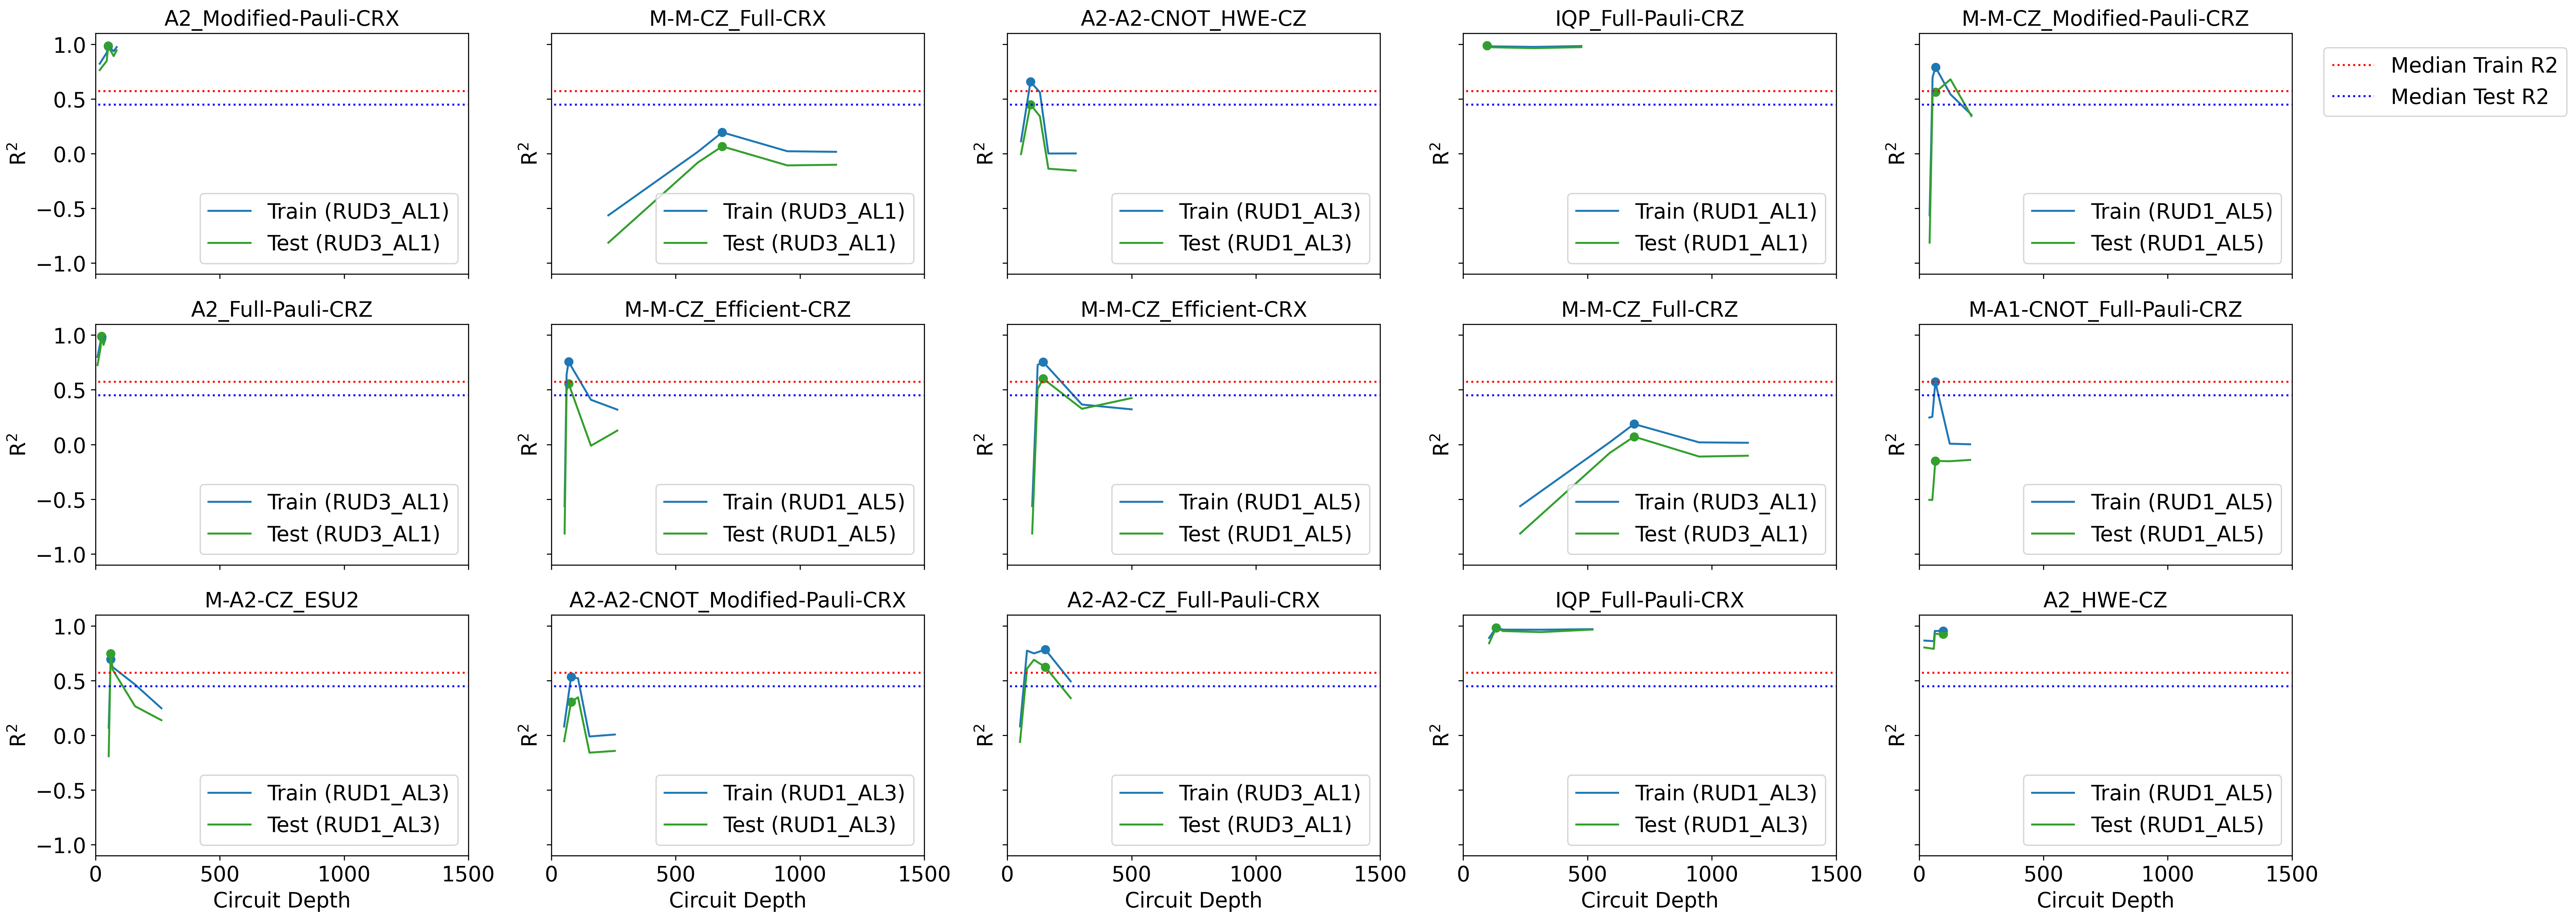
\includegraphics[width=\linewidth]{../images/Function_Fitting/linear_circuitdepth_vs_R2}
		%		\caption{}
		%		\label{fig:linear_circuitdepth_vs_R2}
		%	\end{subfigure}
	%	\hfill		
	\begin{subfigure}[b]{0.49\textwidth}
		\centering
		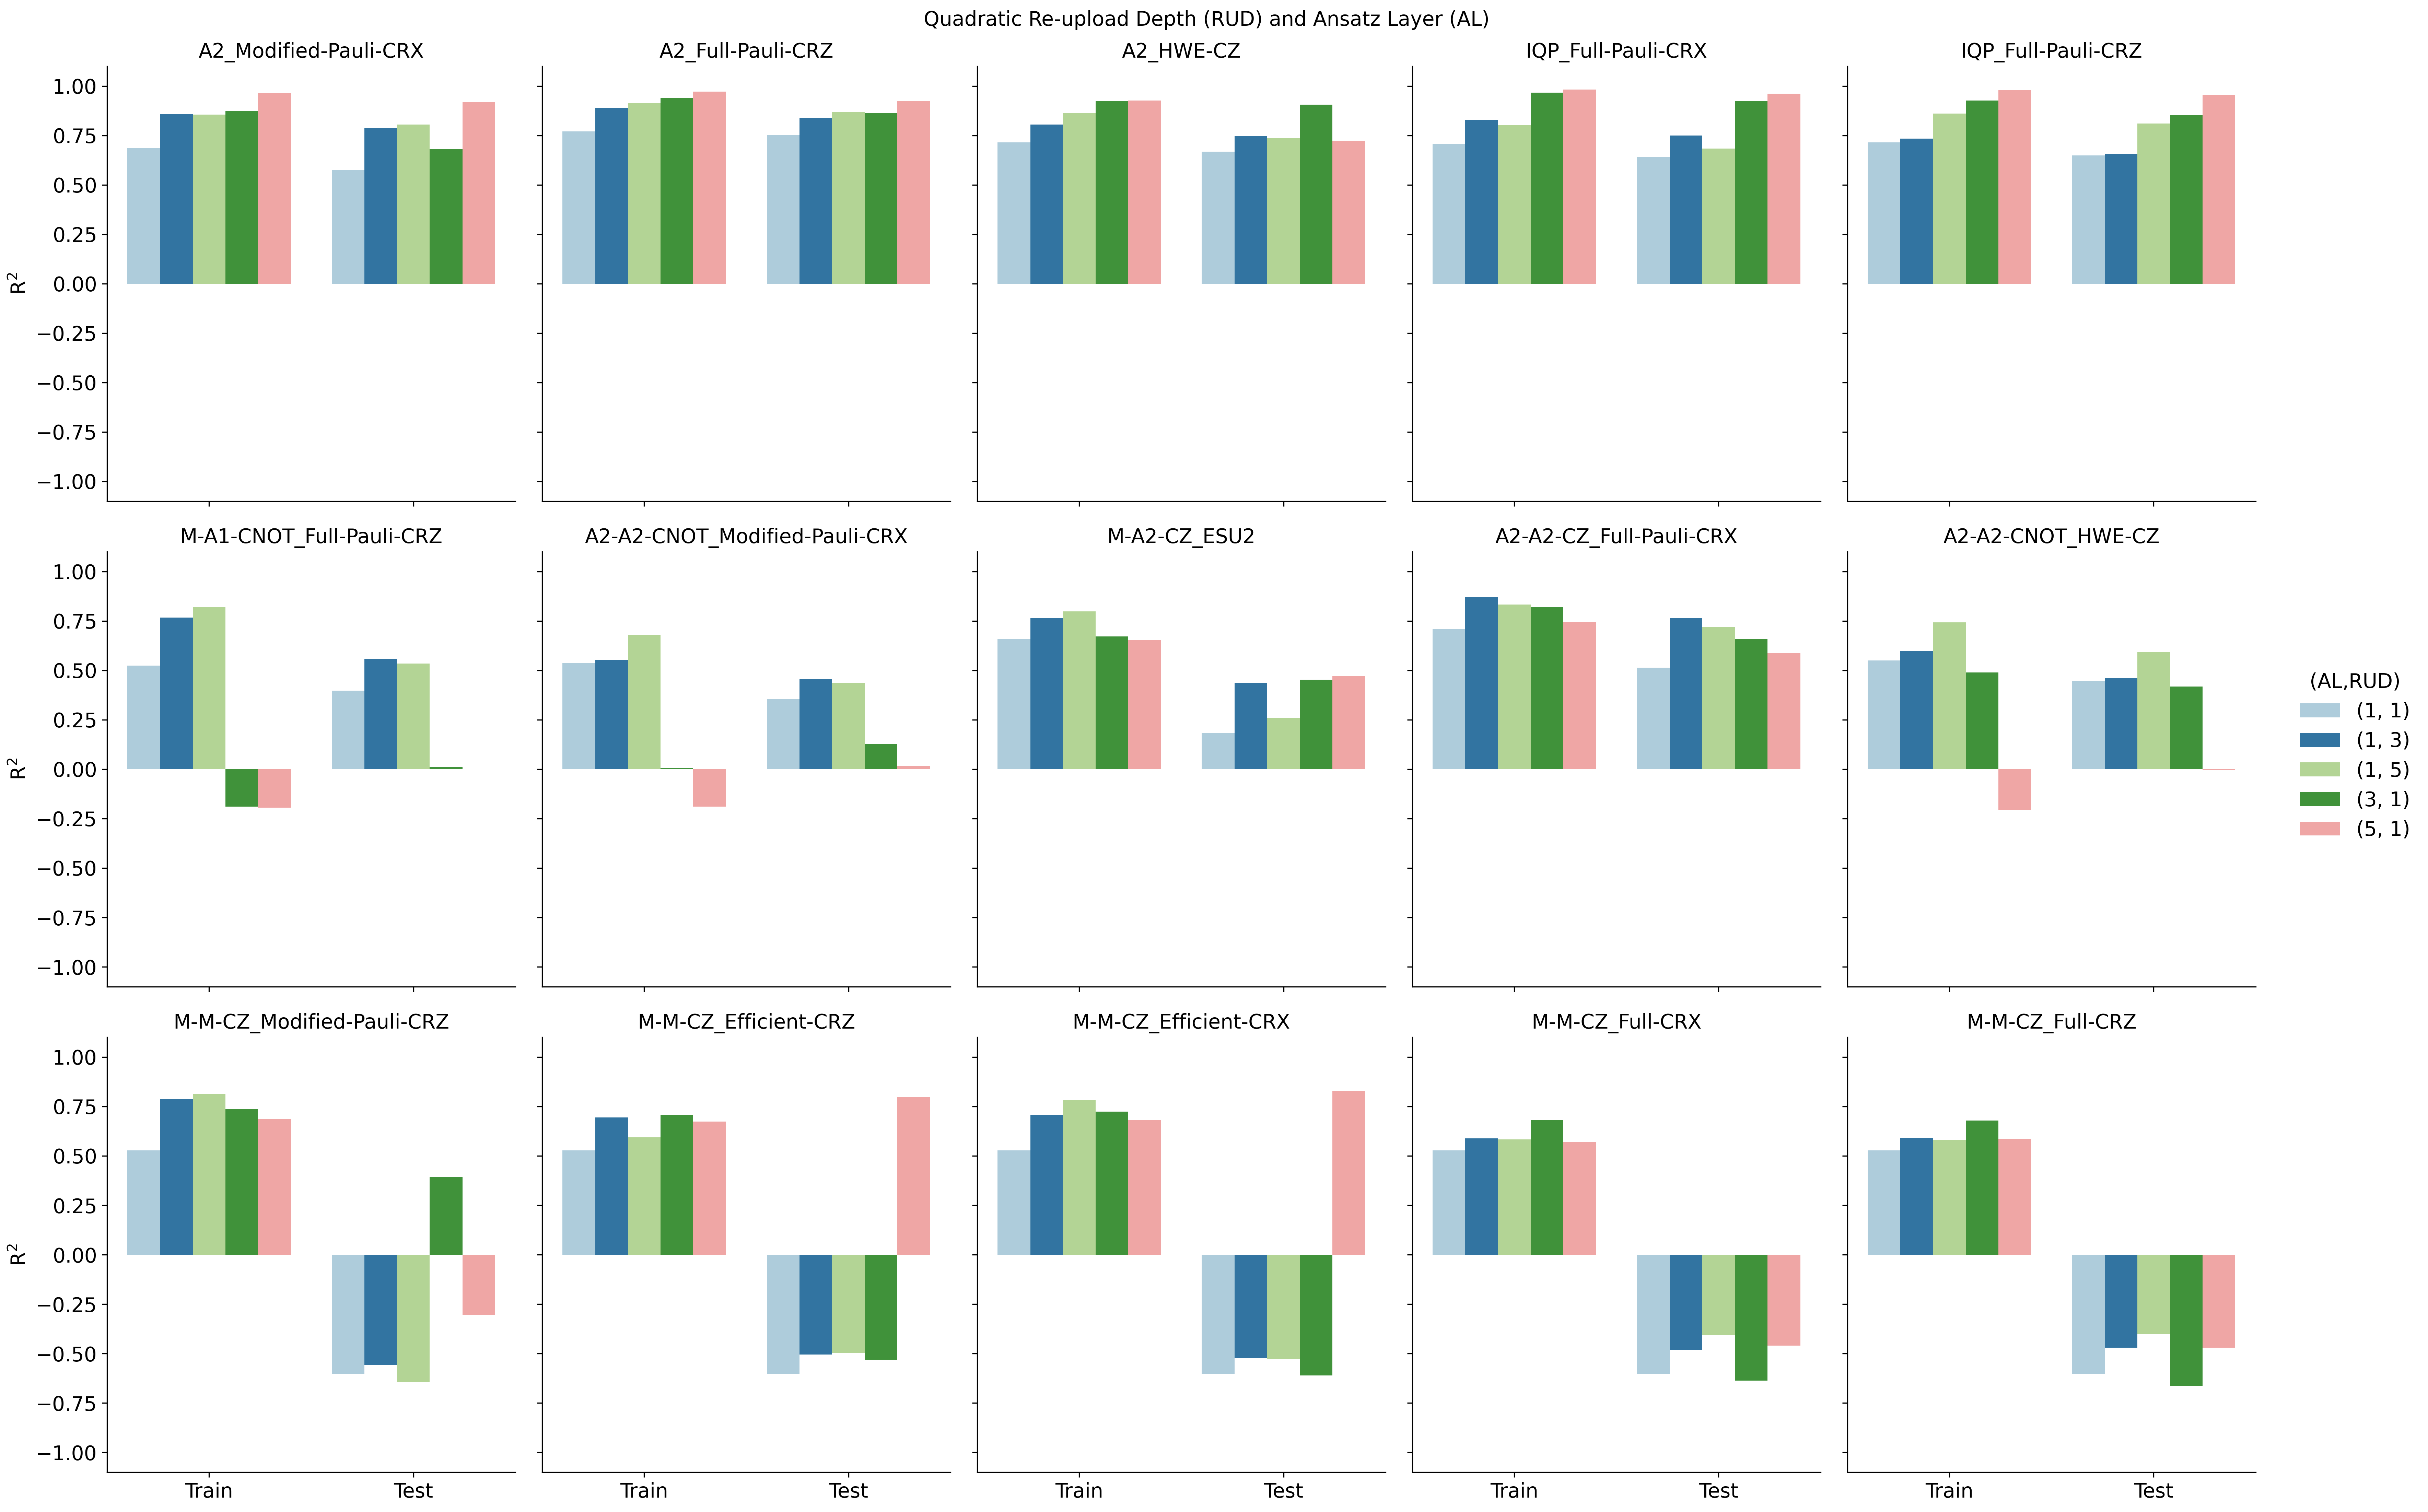
\includegraphics[width=\linewidth]{../images/Function_Fitting/sixteenqubit/16qubit_Quadratic_RUD_AL}
		\caption{}
		\label{fig:16qubit_Quadratic_RUD_AL}
	\end{subfigure}
	\hfill
	%	\begin{subfigure}[b]{0.49\textwidth}
		%		\centering
		%		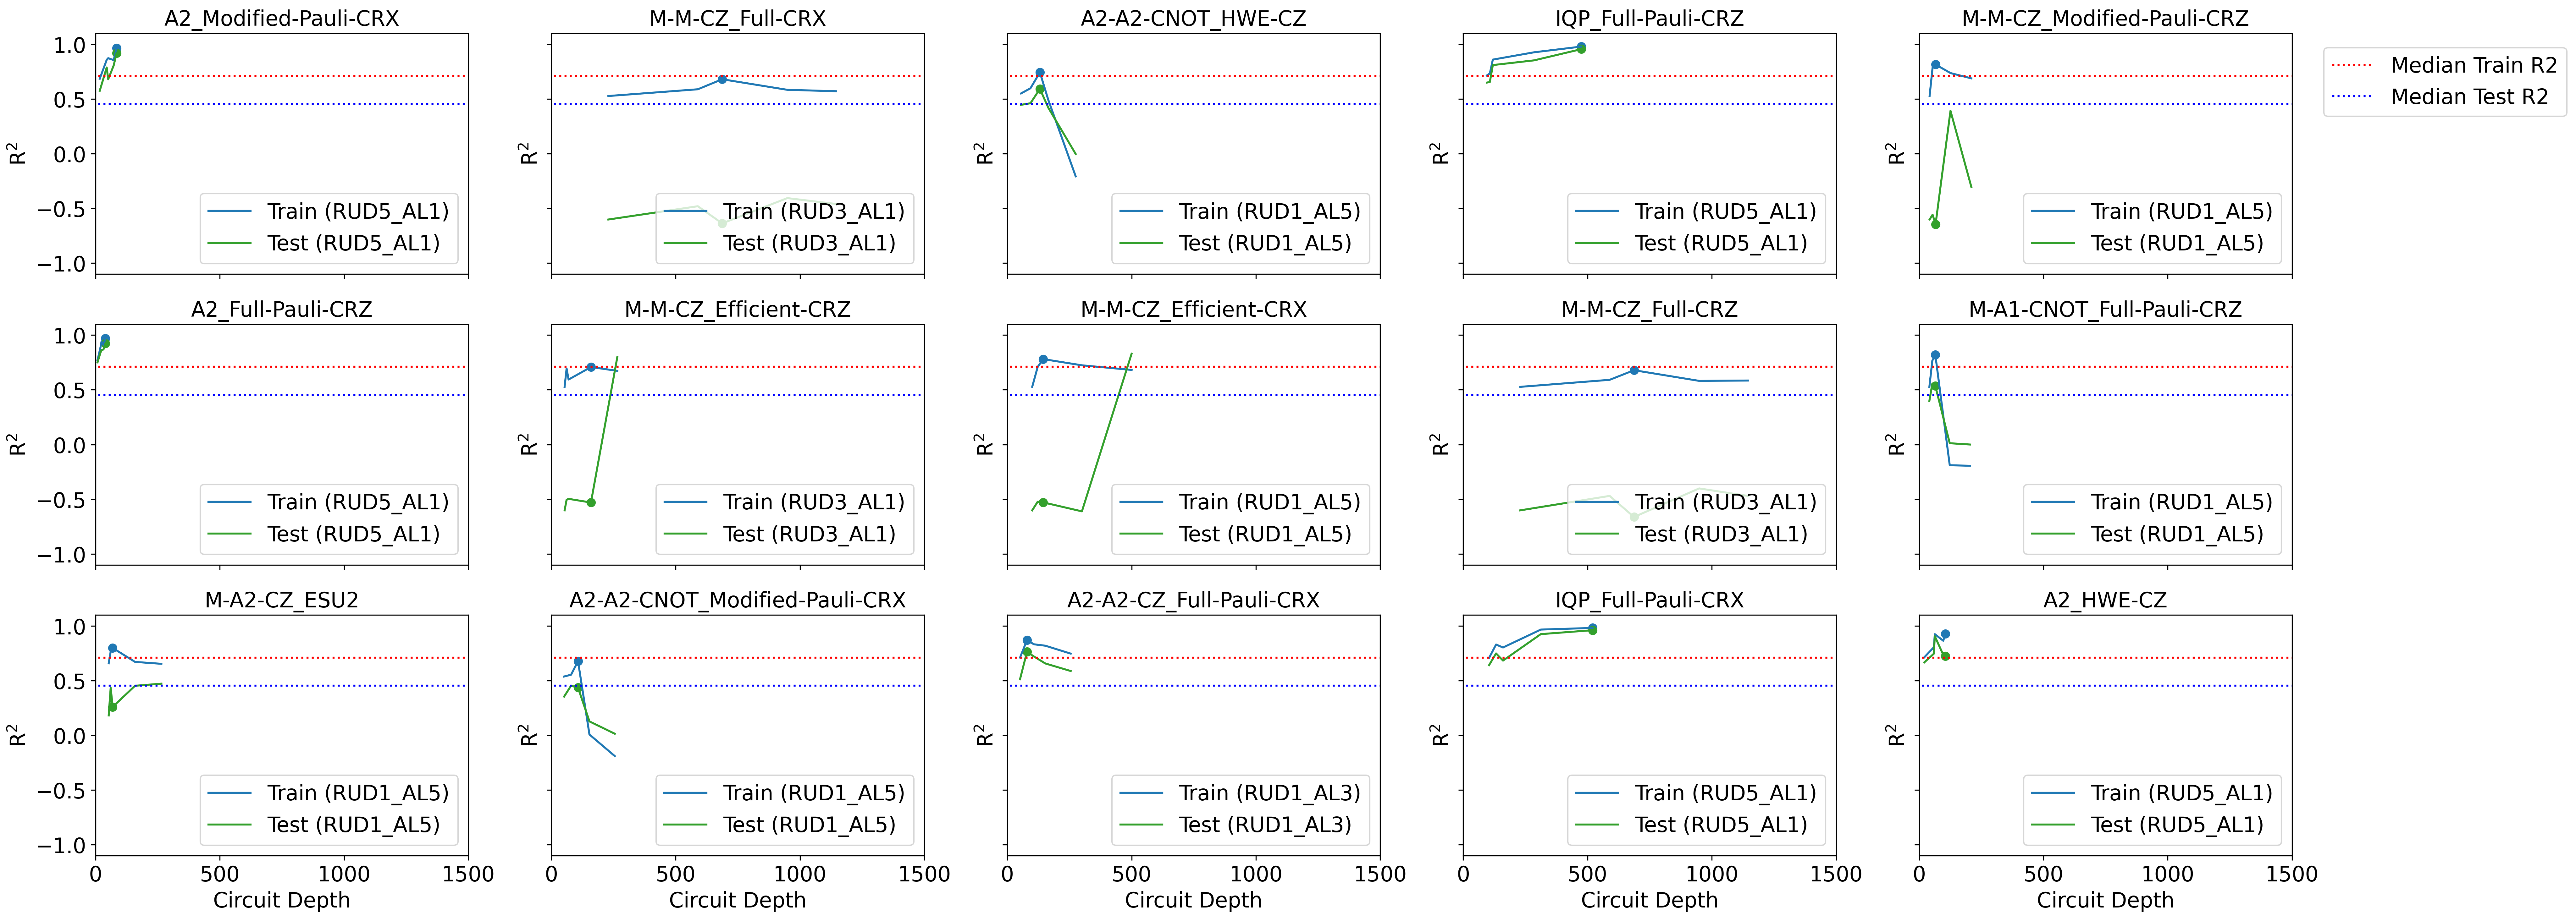
\includegraphics[width=\linewidth]{../images/Function_Fitting/quadratic_circuitdepth_vs_R2}
		%		\caption{}
		%		\label{fig:quadratic_circuitdepth_vs_R2}
		%	\end{subfigure}
	%	\hfill		
	\begin{subfigure}[b]{0.49\textwidth}
		\centering
		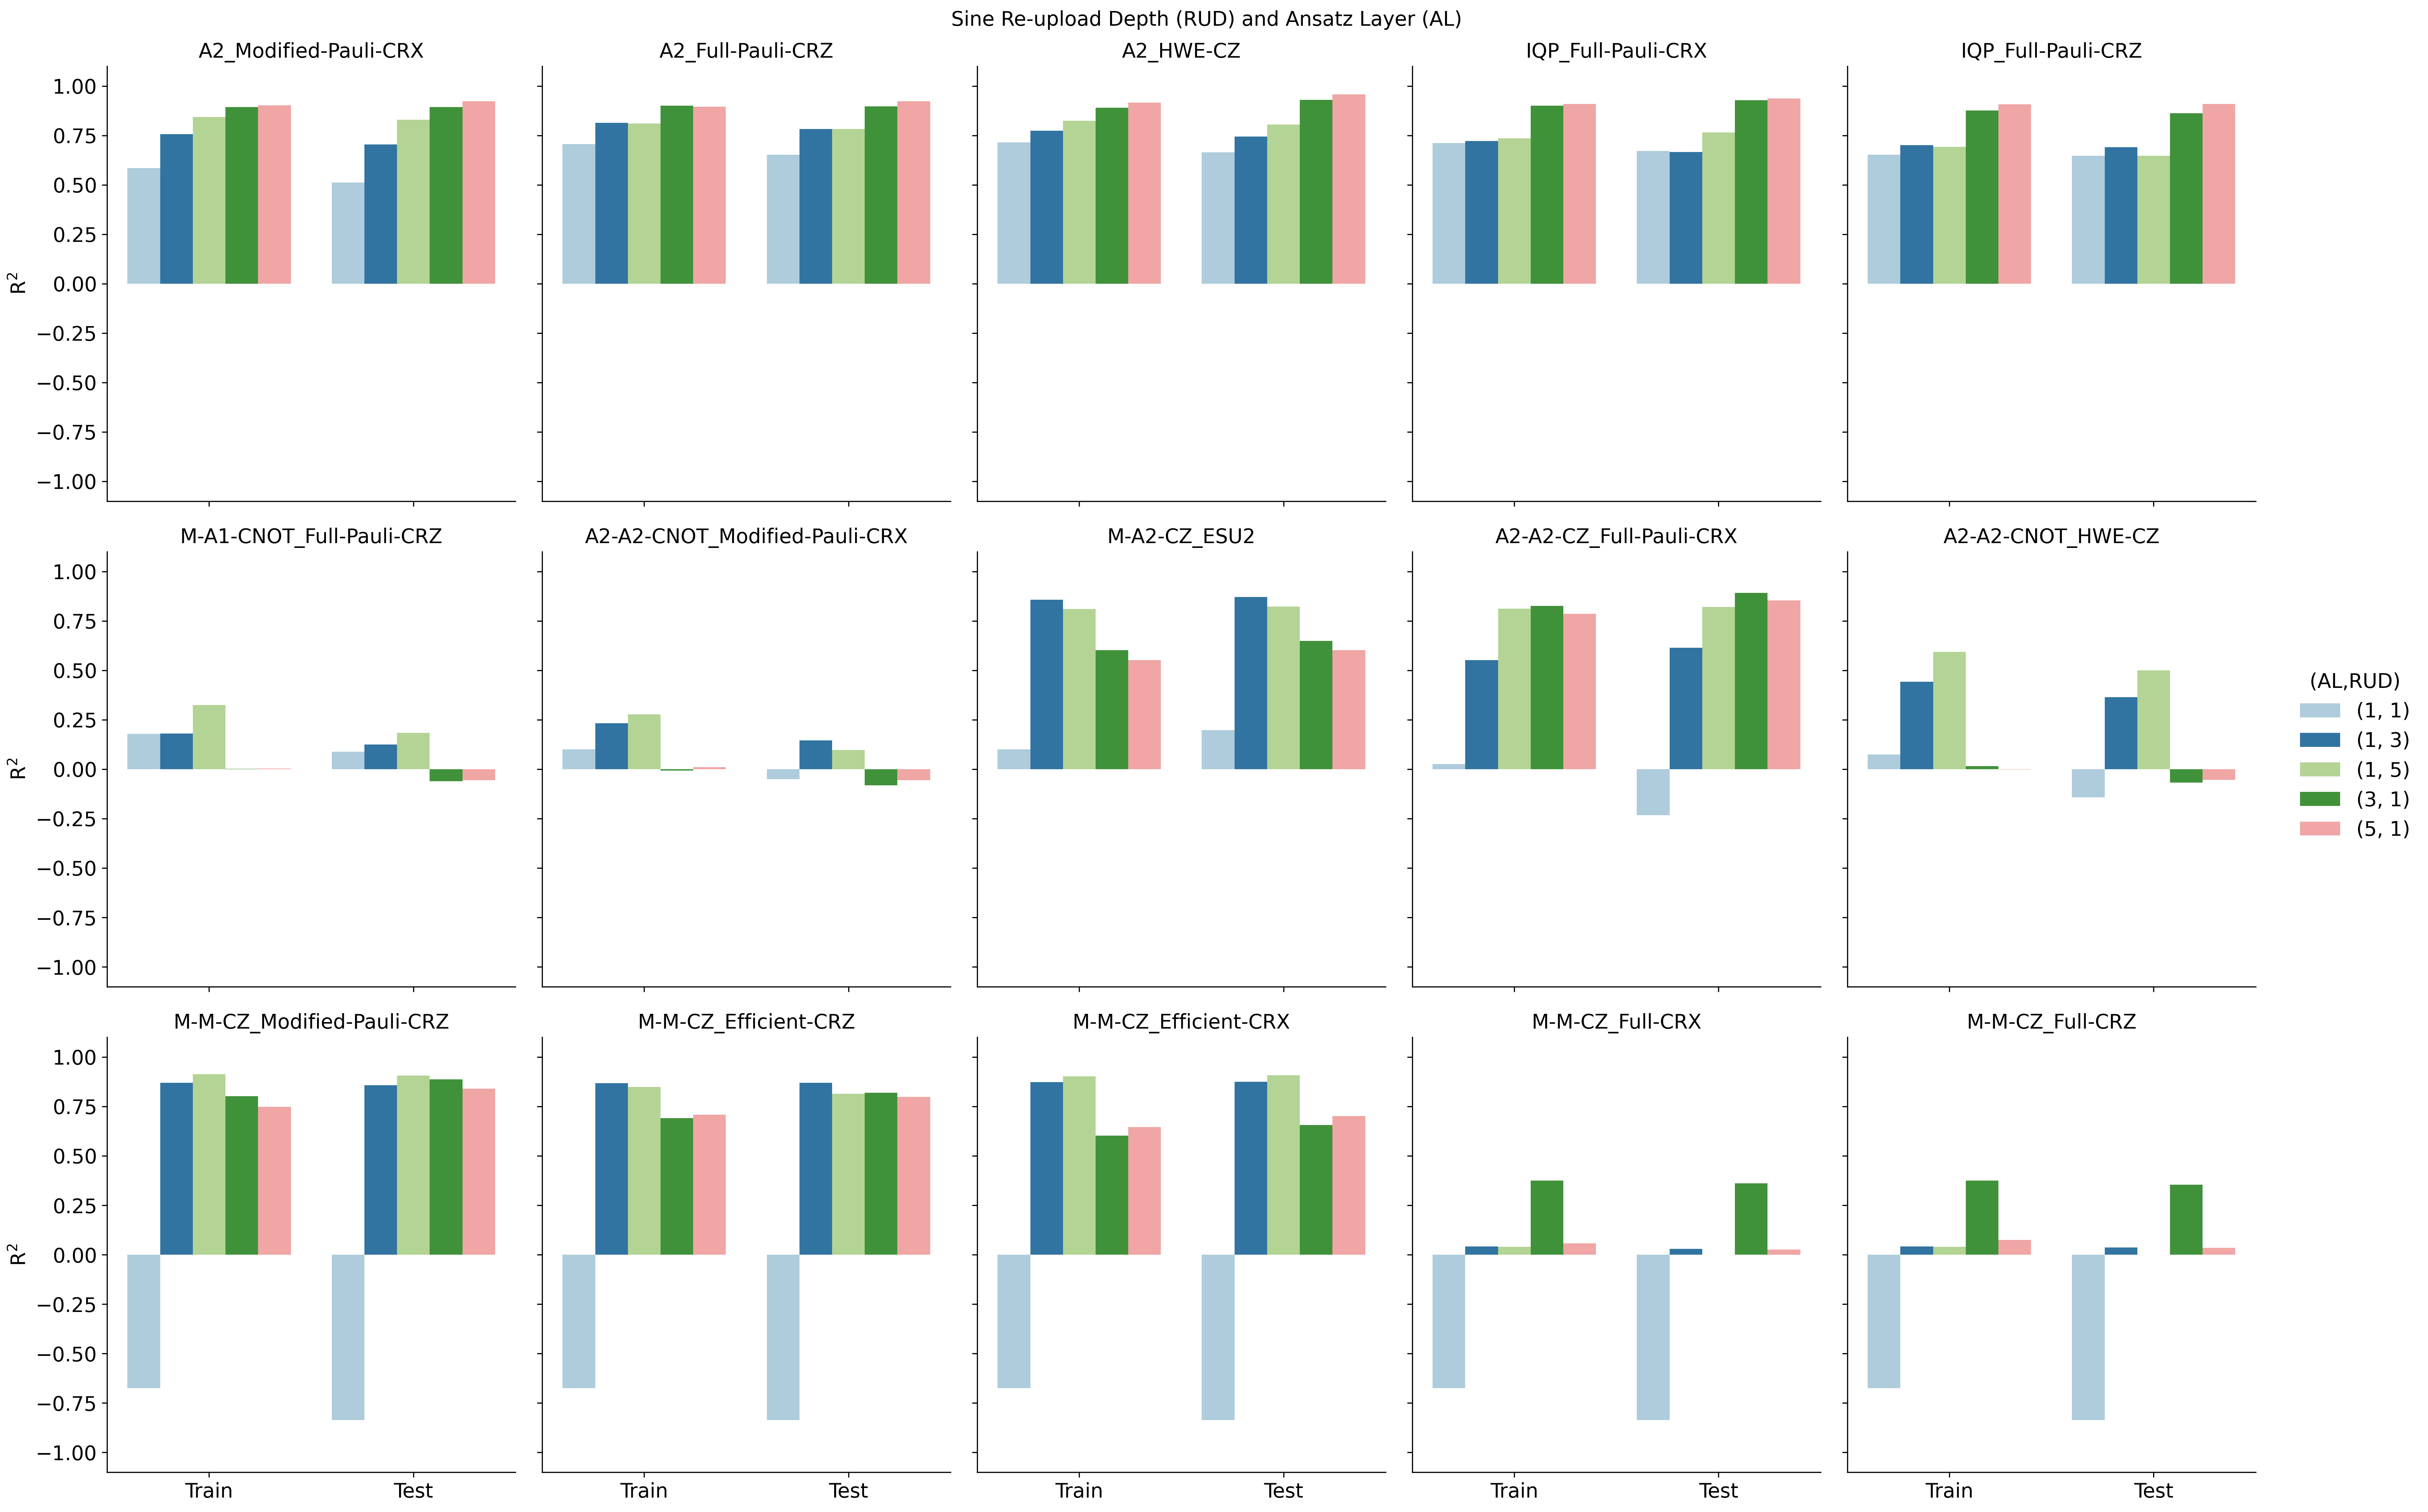
\includegraphics[width=\linewidth]{../images/Function_Fitting/sixteenqubit/16qubit_Sine_RUD_AL.png}
		\caption{}
		\label{fig:16qubit_Sine_RUD_AL}
	\end{subfigure}	
	\hfill
	%	\begin{subfigure}[b]{0.49\textwidth}
		%		\centering
		%		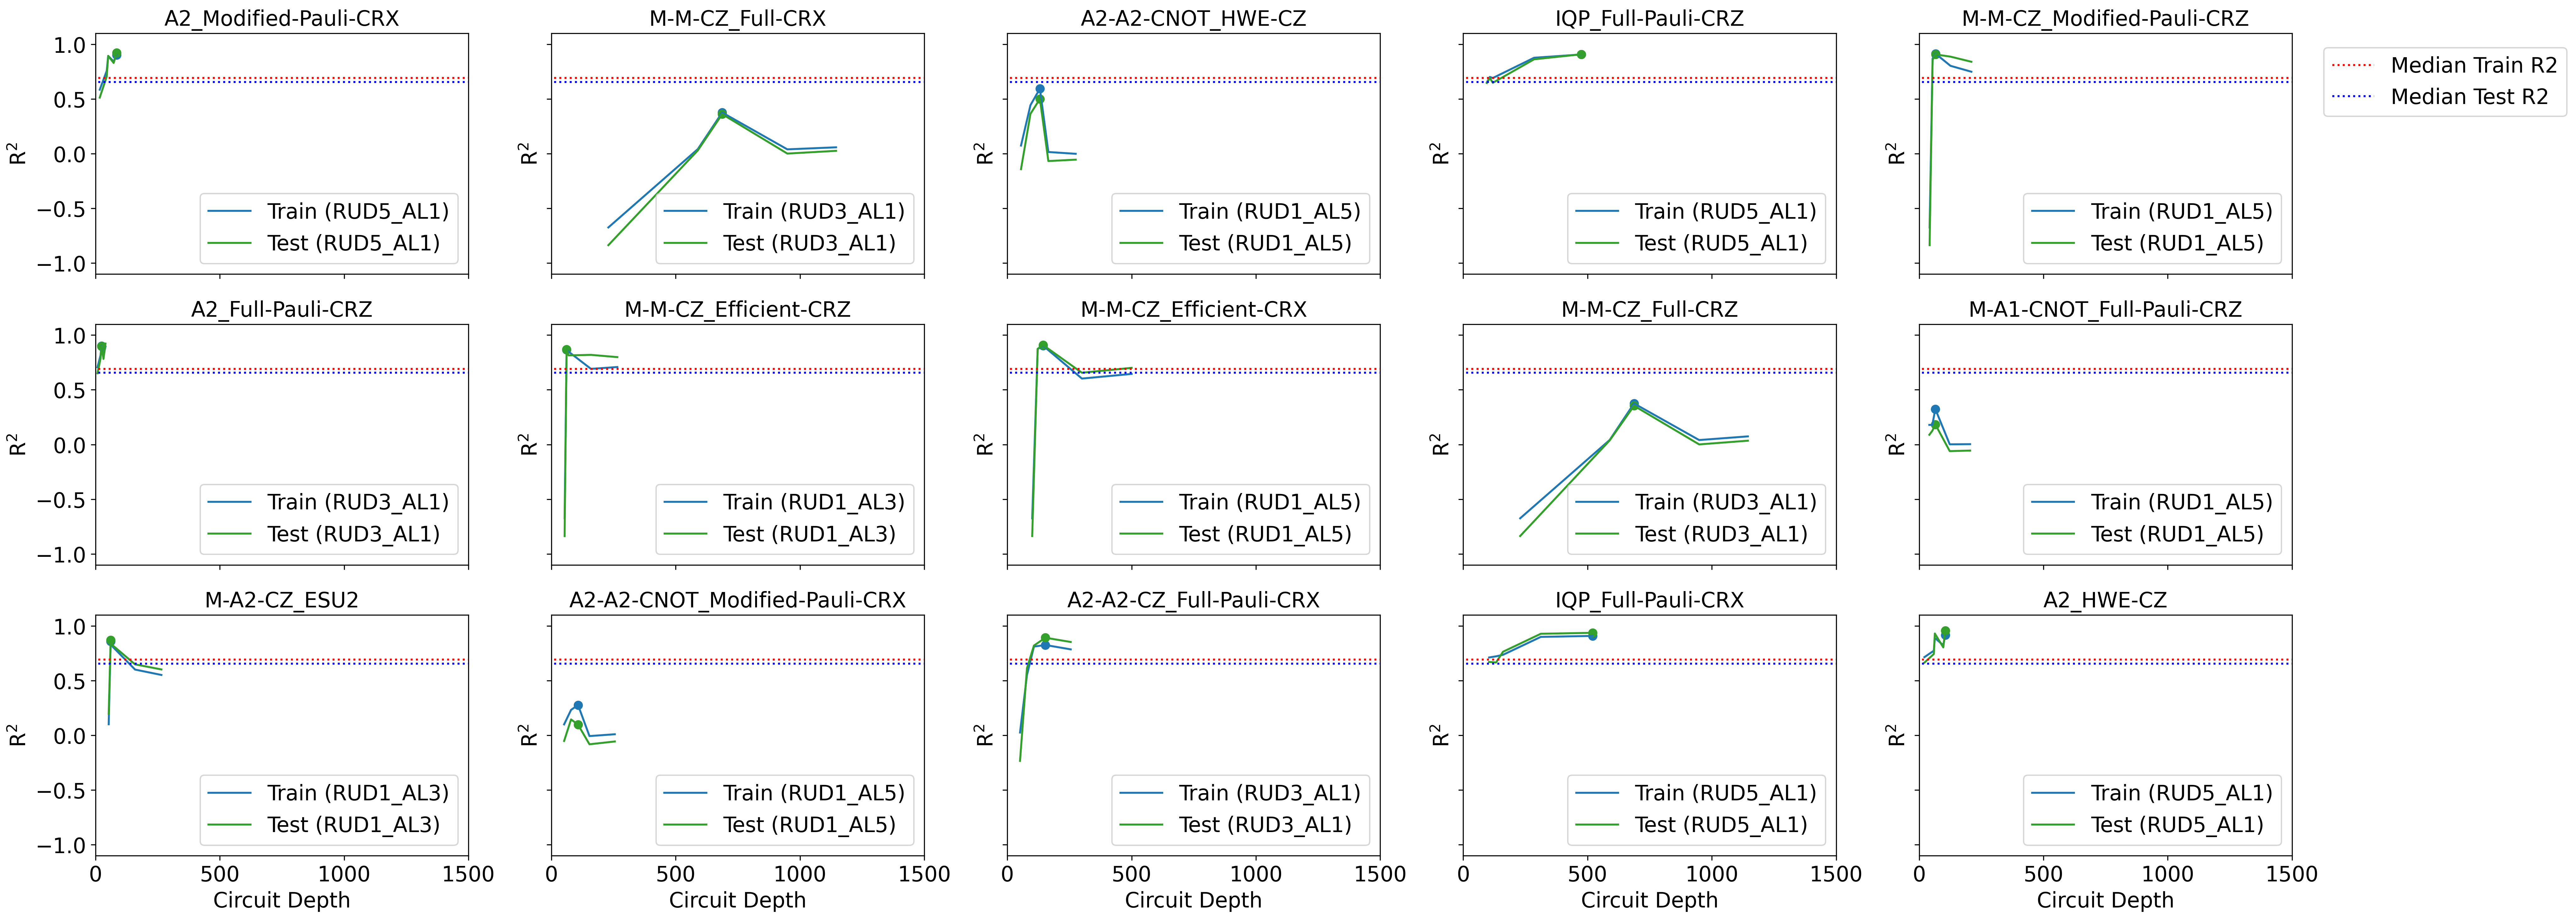
\includegraphics[width=\linewidth]{../images/Function_Fitting/sine_circuitdepth_vs_R2}
		%		\caption{}
		%		\label{fig:sine_circuitdepth_vs_R2}
		%	\end{subfigure}
	%	\hfill		
	\caption{The best five (top row), median five (middle row), and worst five (bottom row) circuits for the 16 qubit (a) linear, (b) quadratic, and (c) sine data show that, in general, an increase in the re-upload depth (RUD) or ansatz layers (AL) increases model performance (R$^{2}$ shown on the y-axis).}
	\label{fig:16qubit_RUD_AL}	
\end{figure}


One proposed advantage of using PQCs for ML tasks is that, in some cases, they can outperform classical ML models using less training data.\cite{hatakeyama-sato_quantum_2023}
We examine this phenomena with learning curves using the best performing circuits previously described.
The learning curves are generated by varying the percentage of training data from 10-80\% of the available data, while holding the number of test points to 10\% of the total data.
The three PQCs for each data set are compared to the classical models mentioned in subsection \ref{subsection:datasets} in a statistical manner (left sub-figures in Figs. \ref{fig:linear_learning_curves}, \ref{fig:quadratic_learning_curves}, and \ref{fig:sine_learning_curves}).
Across the full learning curve, IQP\_Full-Pauli-CRZ (linear function fitting) outperforms seven out of nine classical models for the training set and all of the classical models on the test set.
On the quadratic dataset, using IQP\_Full-Pauli-CRX, offers similar performance to the classical models, despite being outperformed on the training set across the learning curve. 
Similar to the IQP\_Full-Pauli-CRZ using the linear data, IQP\_Full-Pauli-CRX outperforms seven out of the nine classical models on the test set across the full learning curve.
On the sine data, A2\_HWE-CZ is consistent across the learning curve, outperforming six of the nine classical models on the training set and all of the models on the test set.
For all three datasets, this implies that the PQCs offer similar performance to classical models that do well on these datasets but provide better results on the test set.


\begin{figure}[H]
	\centering	
	\begin{subfigure}[b]{0.49\textwidth}
		\centering
		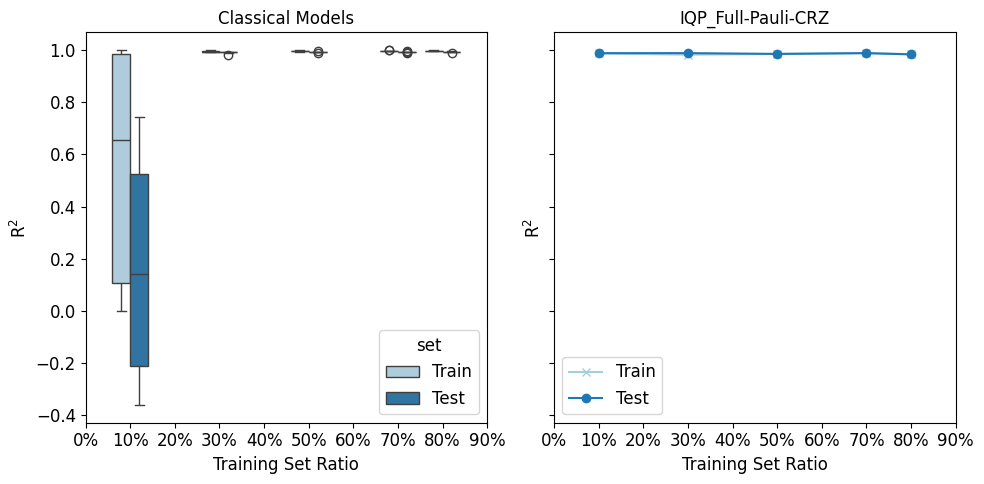
\includegraphics[width=\linewidth]{../images/Function_Fitting/linear_learning_curves.png}
		\caption{}
		\label{fig:linear_learning_curves}
	\end{subfigure}
	\hfill	
	\begin{subfigure}[b]{0.49\textwidth}
		\centering
		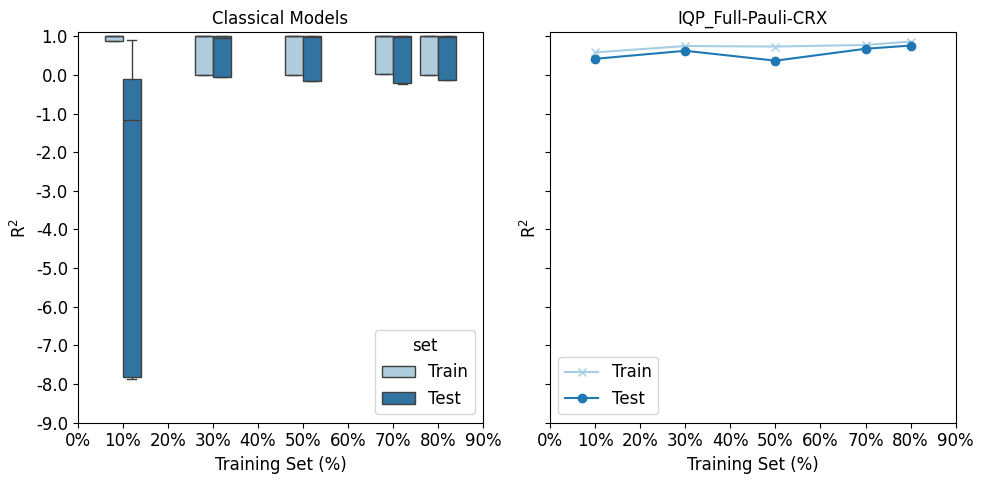
\includegraphics[width=\linewidth]{../images/Function_Fitting/quadratic_learning_curves.png}
		\caption{}
		\label{fig:quadratic_learning_curves}
	\end{subfigure}
	\hfill
	\begin{subfigure}[b]{0.49\textwidth}
		\centering
		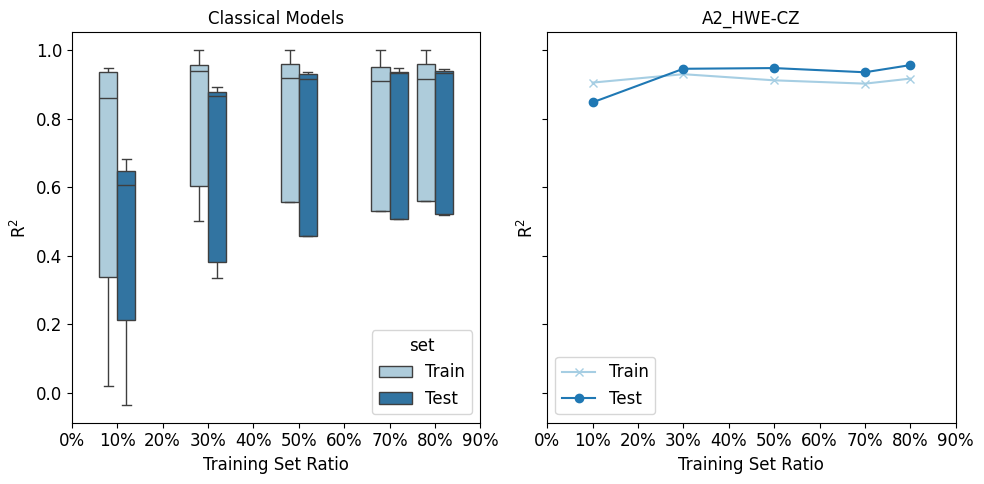
\includegraphics[width=\linewidth]{../images/Function_Fitting/sine_learning_curves.png}
		\caption{}
		\label{fig:sine_learning_curves}
	\end{subfigure}	
	\caption{Learning curves of the best PQCs (right side in the subfigures) versus various classical models (left side in the subfigure) for the (a) linear, (b) quadratic, and (c) sine function datasets.}
	\label{fig:functionfitting_learning_curves}	
\end{figure}


optimization level needs to be set to 0!

Lastly, using the function fitting datasets we analyze the effects of error mitigation on the model accuracy by comparing state vector simulations with noisy and error mitigated simulations using the \textit{fake\_quebec} backend.
Initially, we explored two different methods of error mitigation zero-noise extrapolation (ZNE) using MITIQ\cite{larose_mitiq_2022} and TREX, as implemented in Qiskit. 
We found that both linear and Richardson ZNE were too costly to simulate on classical computers using 16 qubits for all three function fitting datasets and chose only to use TREX for error mitigation.
Our analysis revealed that the state vector, TREX, and unmitigated IQP\_Full-Pauli-CRZ (linear function fitting data) models all have R$^{2}$ between 0.98 and 0.99, for both the training and test sets, as highlighted in Fig. \ref{fig:linear_error_mitigation}.
While the performance of the linear data can be attributed to the simiplicity of the dataset, for the quadratic function fitting data using IQP\_Full-Pauli-CRX (Fig. \ref{fig:quadratic_error_mitigation}), we found that the model with unmitigated error has an R$^{2}$ of 0.65 for the training set and 0.45 for the test set.
This model is improved slightly by the incorporation of error mitigation using TREX, where the training set R$^{2}$ is 0.69 and test set R$^{2}$ is 0.60.
Overall, the model using TREX offers results more comparable to the state vector simulations, which has a R$^{2}$s of 0.80 and 0.68 for the training and test set, respectively.
On the sine function fitting data, using A2\_HWE-CZ (Fig. \ref{fig:sine_error_mitigation}), for the state vector, TREX, and unmitigated models, the training sets have R$^{2}$s of 0.92, 0.87, and 0.87, respectively, while the test sets have R$^{2}$s of 0.96, 0.89, and 0.91, respectively.
Overall, while these results are for simple function fitting data, we concluded that TREX offers a computational efficient error mitigation method, with results similar to the state vector calculations.0


\begin{figure}[H]
	\centering	
	\begin{subfigure}[b]{0.49\textwidth}
		\centering
		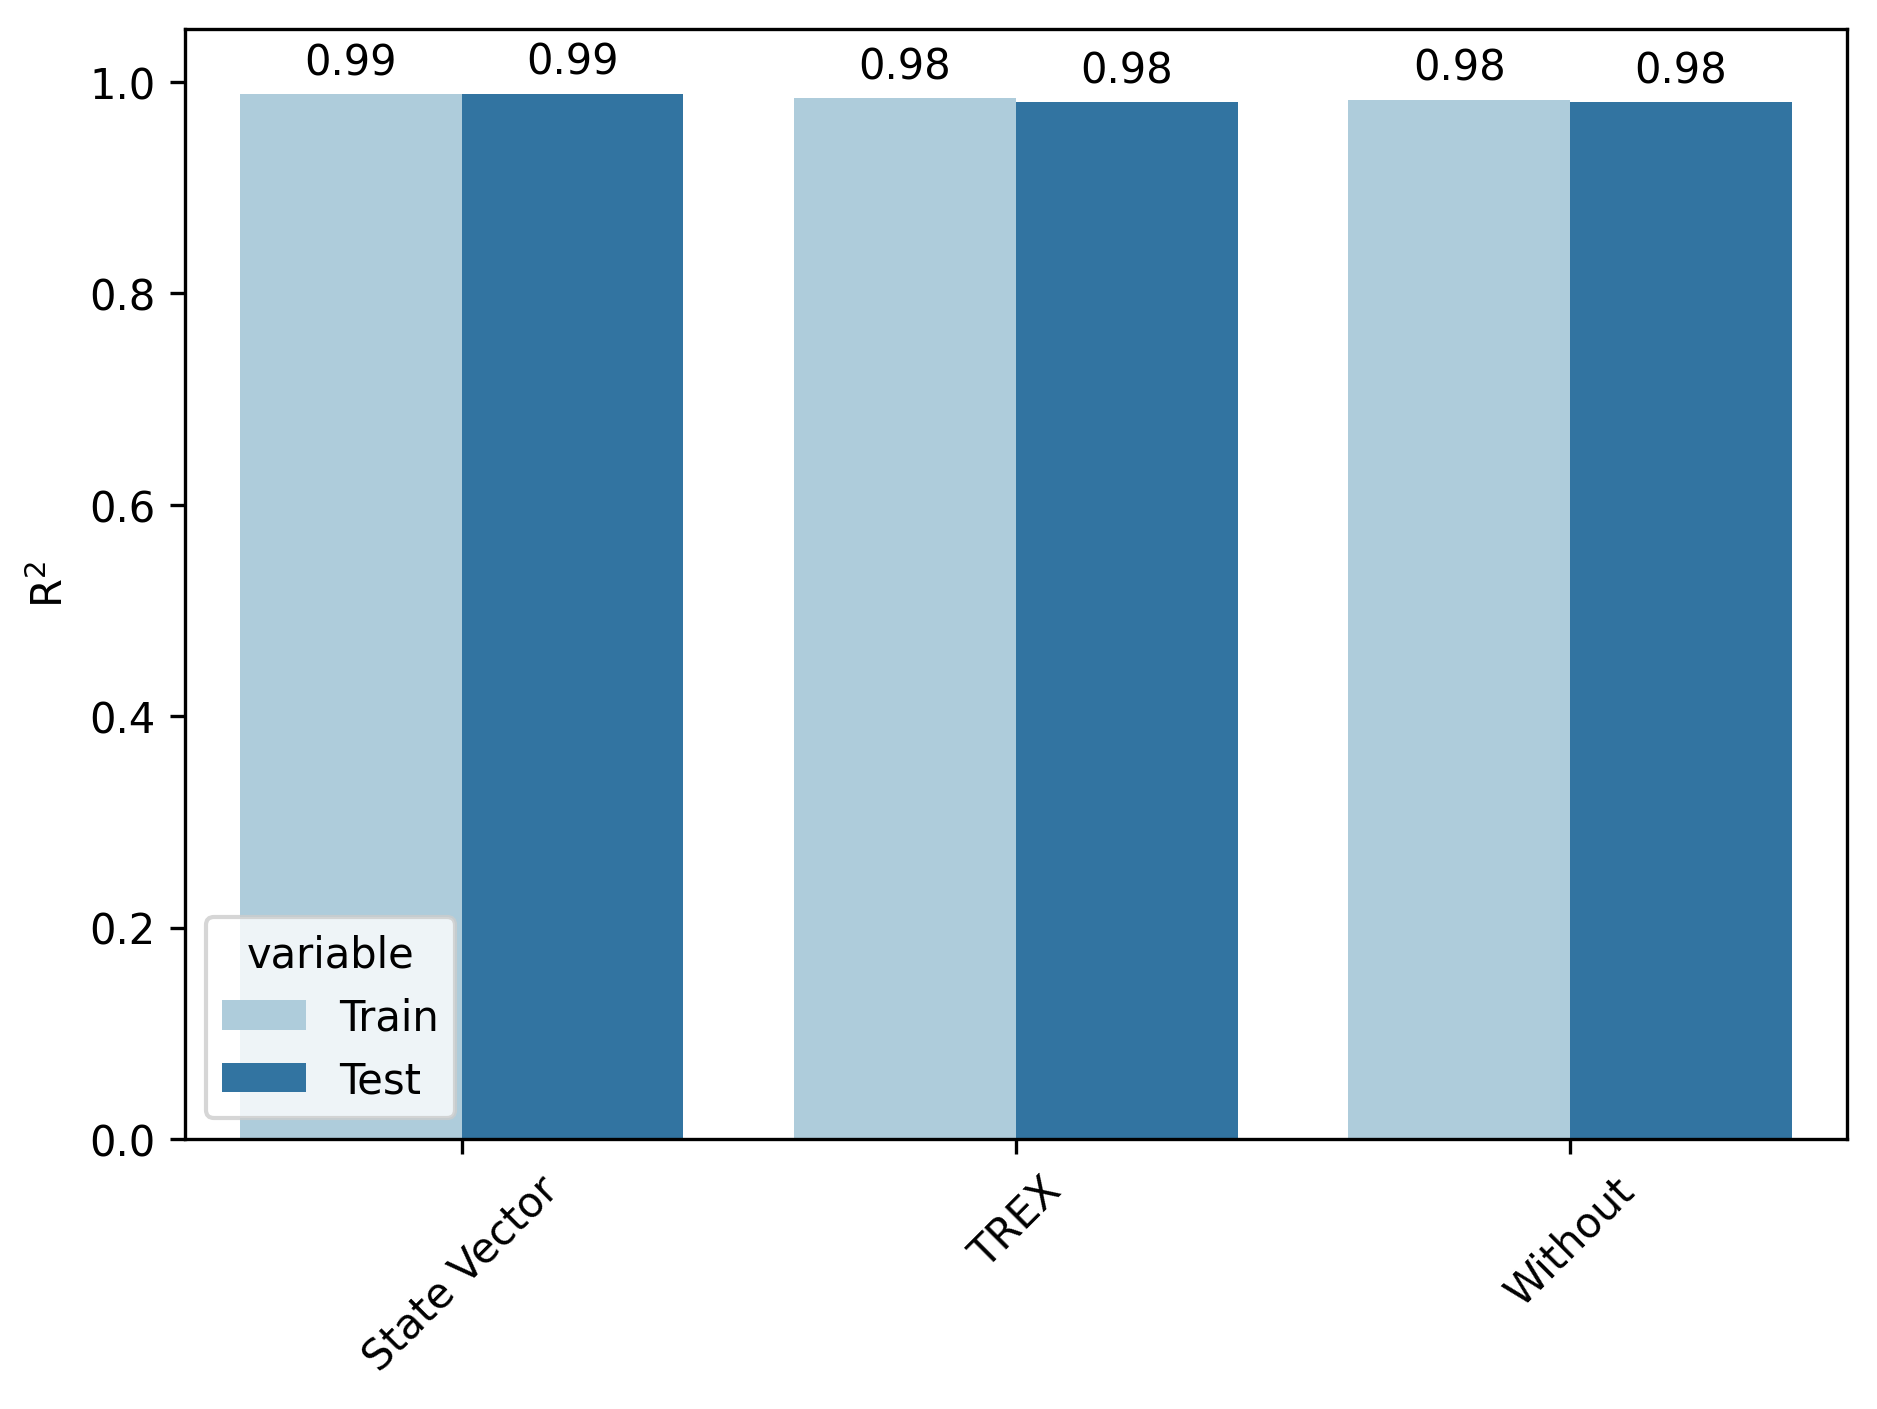
\includegraphics[width=\linewidth]{../images/Function_Fitting/linear_error_mitigation.png}
		\caption{}
		\label{fig:linear_error_mitigation}
	\end{subfigure}
	\hfill	
	\begin{subfigure}[b]{0.49\textwidth}
		\centering
		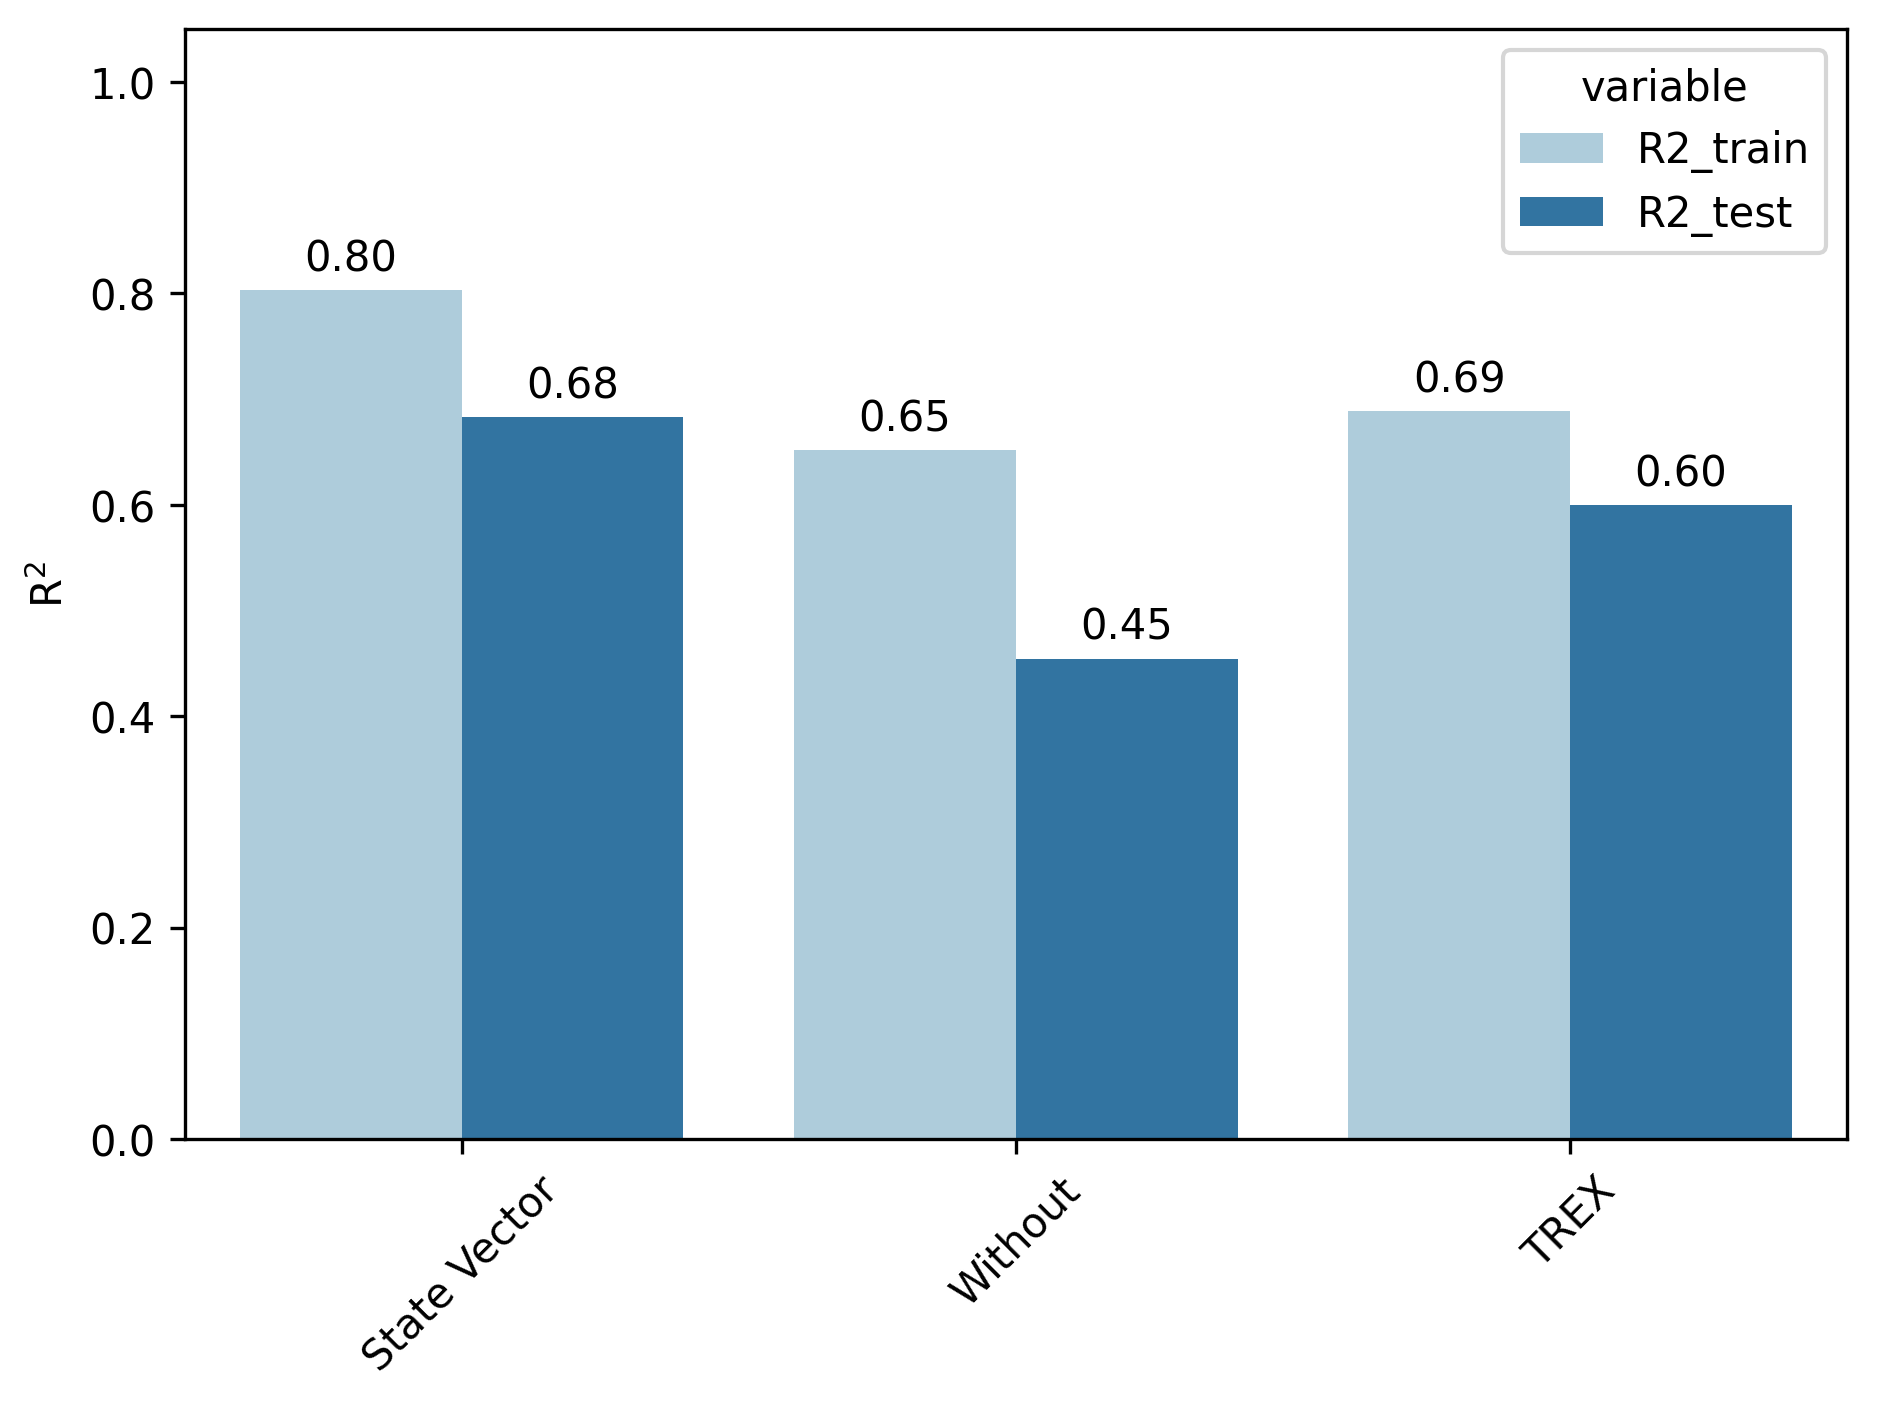
\includegraphics[width=\linewidth]{../images/Function_Fitting/quadratic_error_mitigation.png}
		\caption{}
		\label{fig:quadratic_error_mitigation}
	\end{subfigure}	
	\begin{subfigure}[b]{0.49\textwidth}
		\centering
		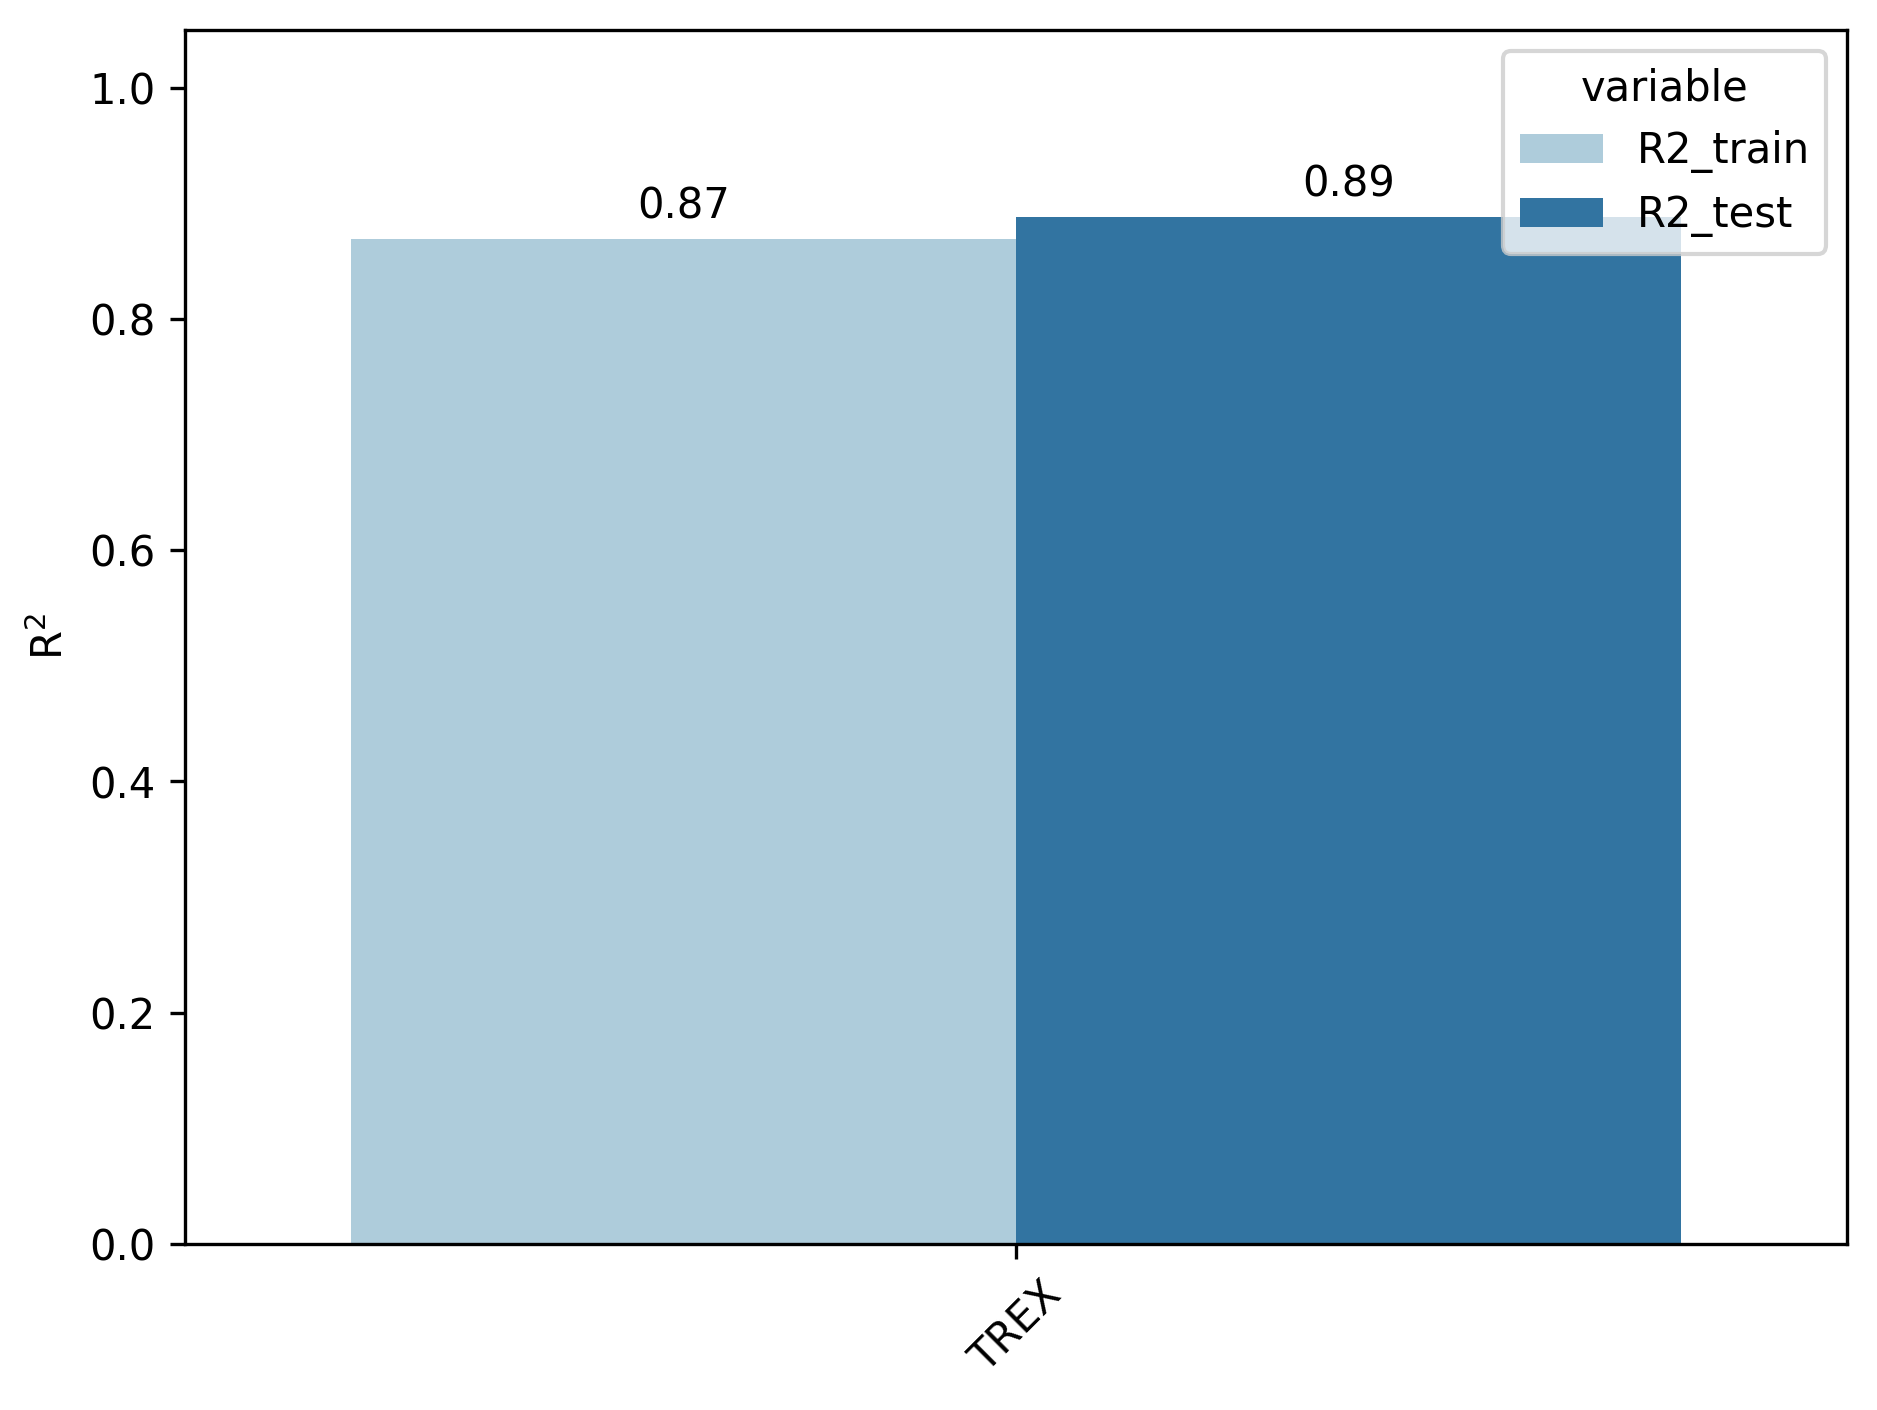
\includegraphics[width=\linewidth]{../images/Function_Fitting/sine_error_mitigation.png}
		\caption{}
		\label{fig:sine_error_mitigation}
	\end{subfigure}
	\hfill		
	\caption{Error mitigation benchmarking for the (a) linear, (b) quadratic, and (c) sine function comparing unmitigated and mitigated error using TREX with state vector simulations.}
	\label{fig:functionfitting_errormitigation}	
\end{figure}



\bibliography{achemso-demo}

\end{document}